W dwa lata za Bolesławą przyszedł na świat Franciszek Głąb (ur. 2 VIII 1910~r. w Mirowie) (ryc.~\ref{rys:akt_urodzenia_franciszka_glaba}).

\begin{figure}
\begin{center}
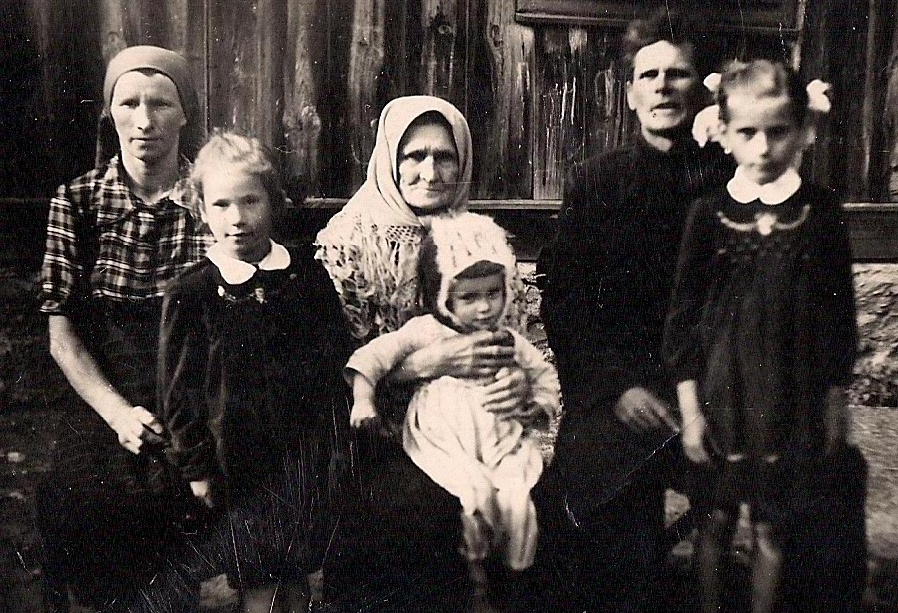
\includegraphics[width=0.75\textwidth]{zdjecia/rodzina_eleonory_franciszka_glabow.jpg}
\caption[Rodzina Franciszka i Eleonory Głąbów z babcią Antoniną]{Na zdjęciu od lewej: Eleonora Głąb z domu Merta, Czesława Głąbianka, babcia Antonina Głąb z wnuczkiem Mirosławem Głąbem, Franciszek Głąb i Mirosława Głąbianka}
\label{rys:rodzina_eleonory_franciszka_glabow}
\end{center}
\end{figure}

\begin{figure}
\begin{center}
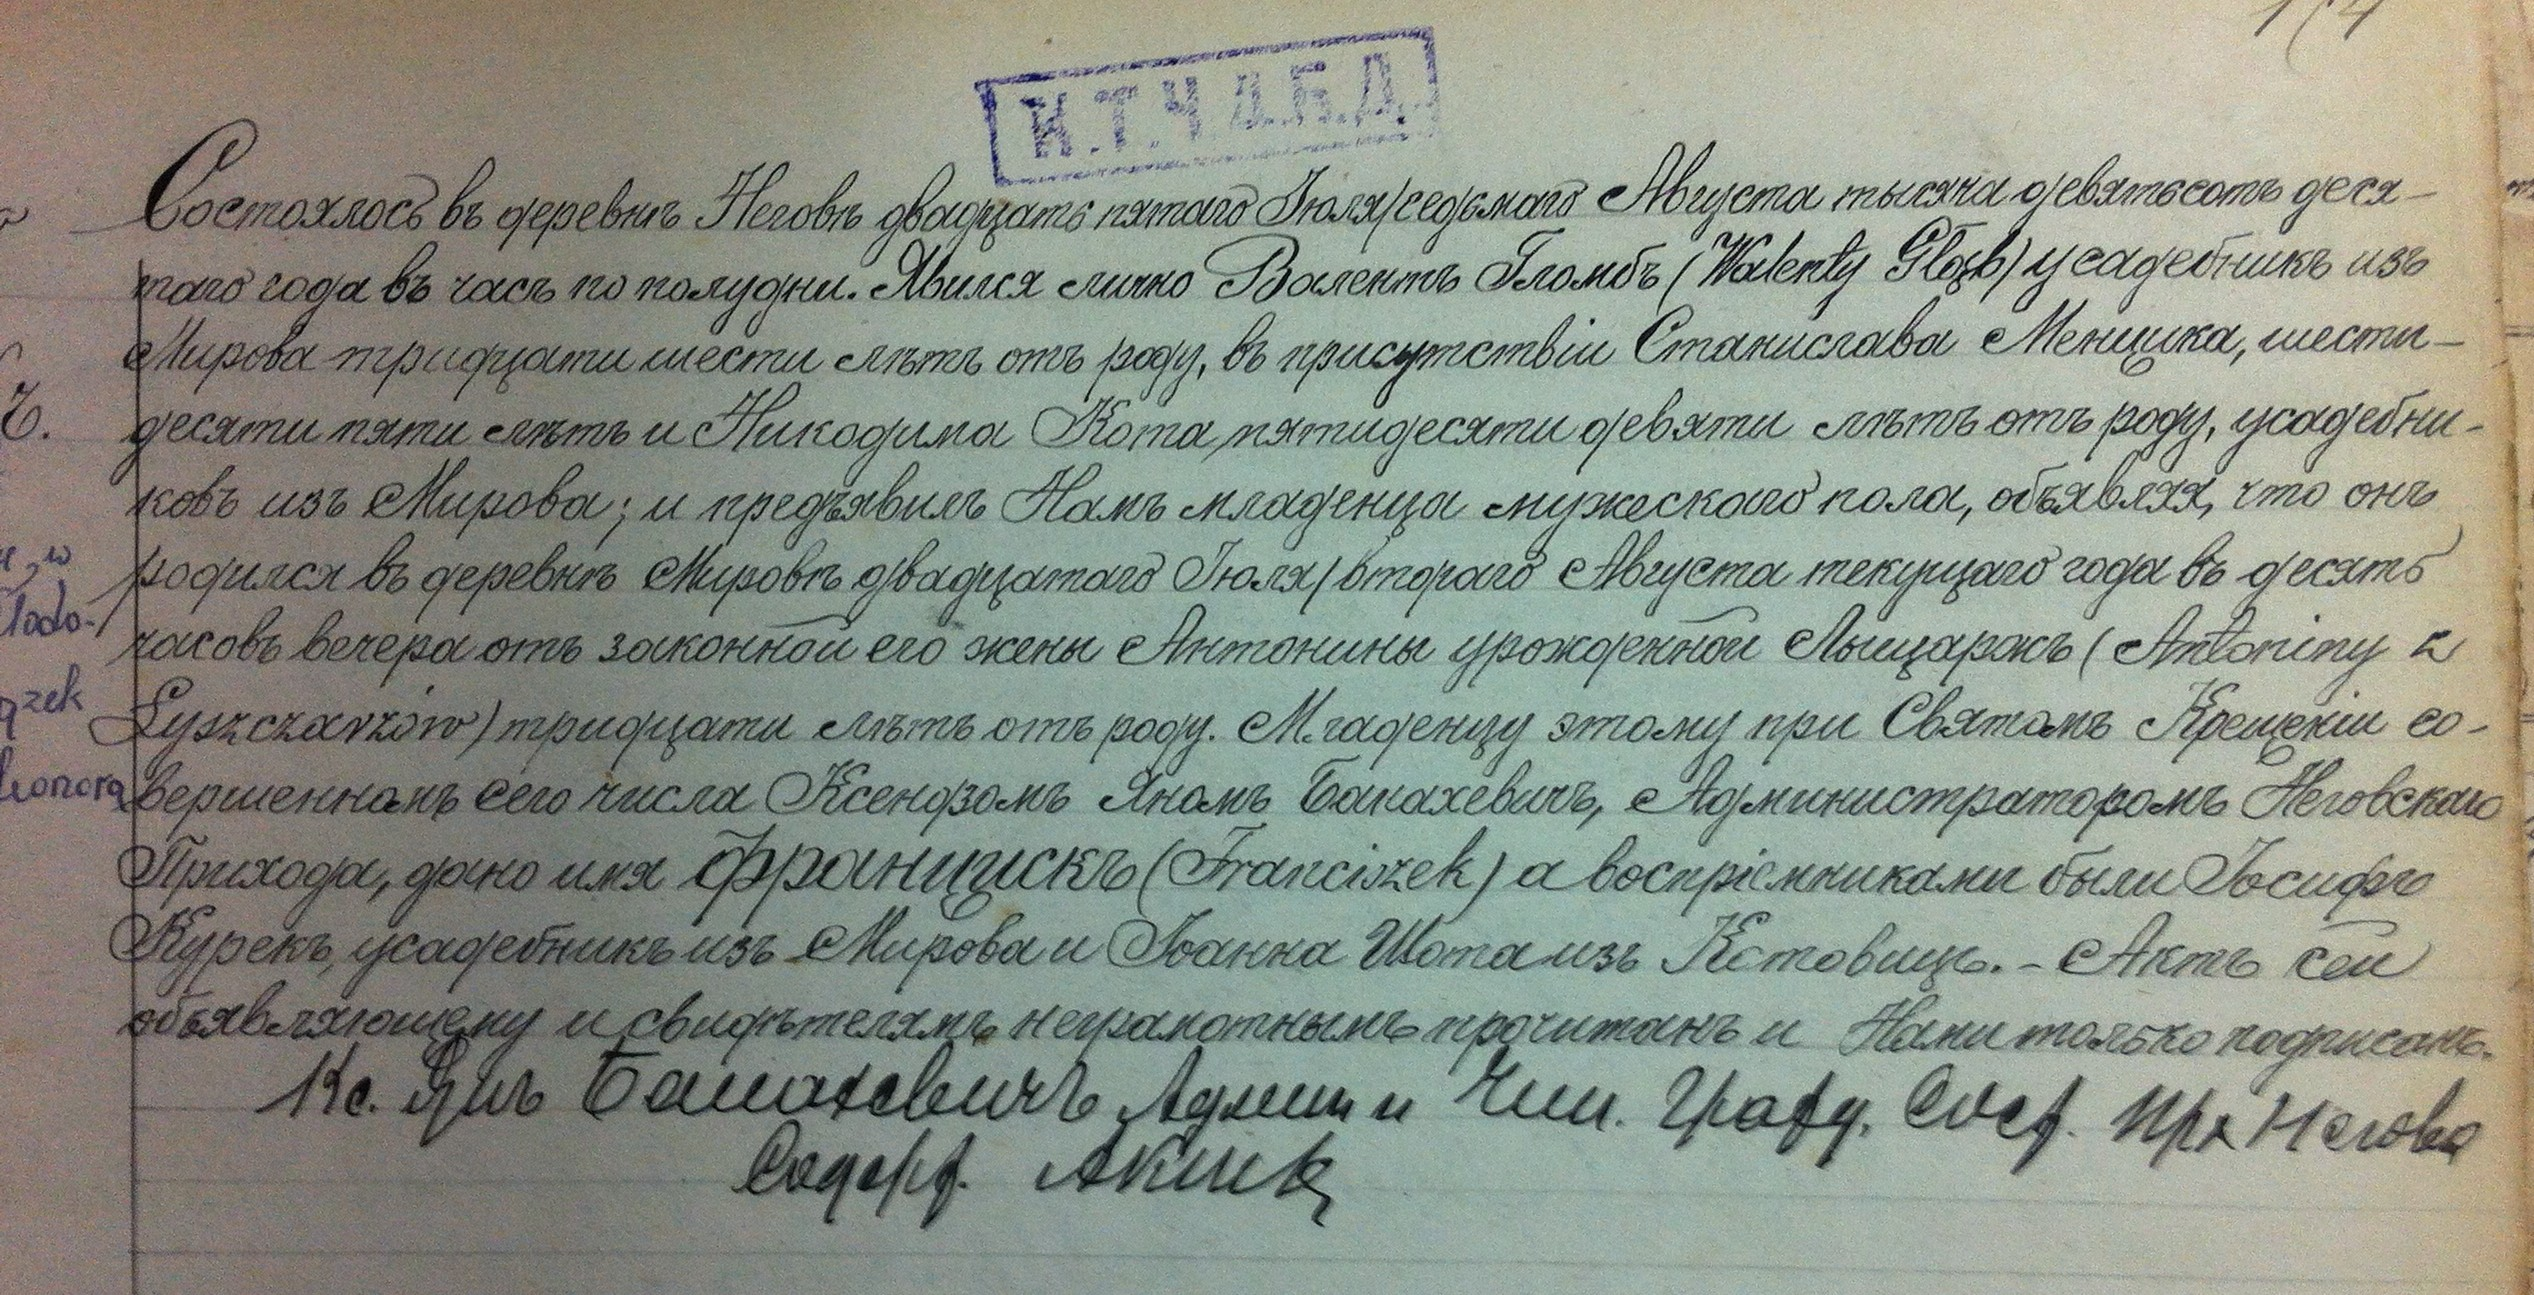
\includegraphics[width=\textwidth]{zdjecia/akt_urodzenia_franciszka_glaba.jpg}
\caption{Akt urodzenia Franciszka Głąba}
\label{rys:akt_urodzenia_franciszka_glaba}
\end{center}
\end{figure}



Po wojnie, którą przeżył na robotach przymusowych w Niemczech, ożenił się we Włodowicach 25 stycznia 1948~r. z Eleonorą Mertą (ur. 1 I 1915~r. w Górze Włodowskiej, córką Piotra i Stanisławy z domu Opałko). Był to ostatni ślub w rodzinie Walentego i Antoniny Głąbów. Doczekał się z nią piątki dzieci: córki Mirosławy (ur. 10 XI 1948~r. w Mirowie), córki Czesławy (ur. w Mirowie 18 XI 1950~r.), córki Barbary (ur. 19 XII 1952~r. w Mirowie), która z woli ojca Franciszka została oddana na wychowanie jego bezdzietnej siostrze Anieli Głąb Biskupskiej mieszkającej w Ligocie Dolnej koło Kluczborka, syna Mirosława, jak się okazuje, najmłodszego żyjącego wnuka Walentego i Antoniny (ur. 21 VI 1954~r. w Mirowie) oraz syna Bogusława Jarosława (ur. 1 X 1957~r. w Mirowie), który podczas pożaru Mirowa przeziębił się i doznał zapalenia opon mózgowych, co spowodowało jego śmierć 12 V 1958~r. w Myszkowie.





\section{Mirosława Jabłońska z domu Głąb}
   
\begin{figure}
\begin{center}
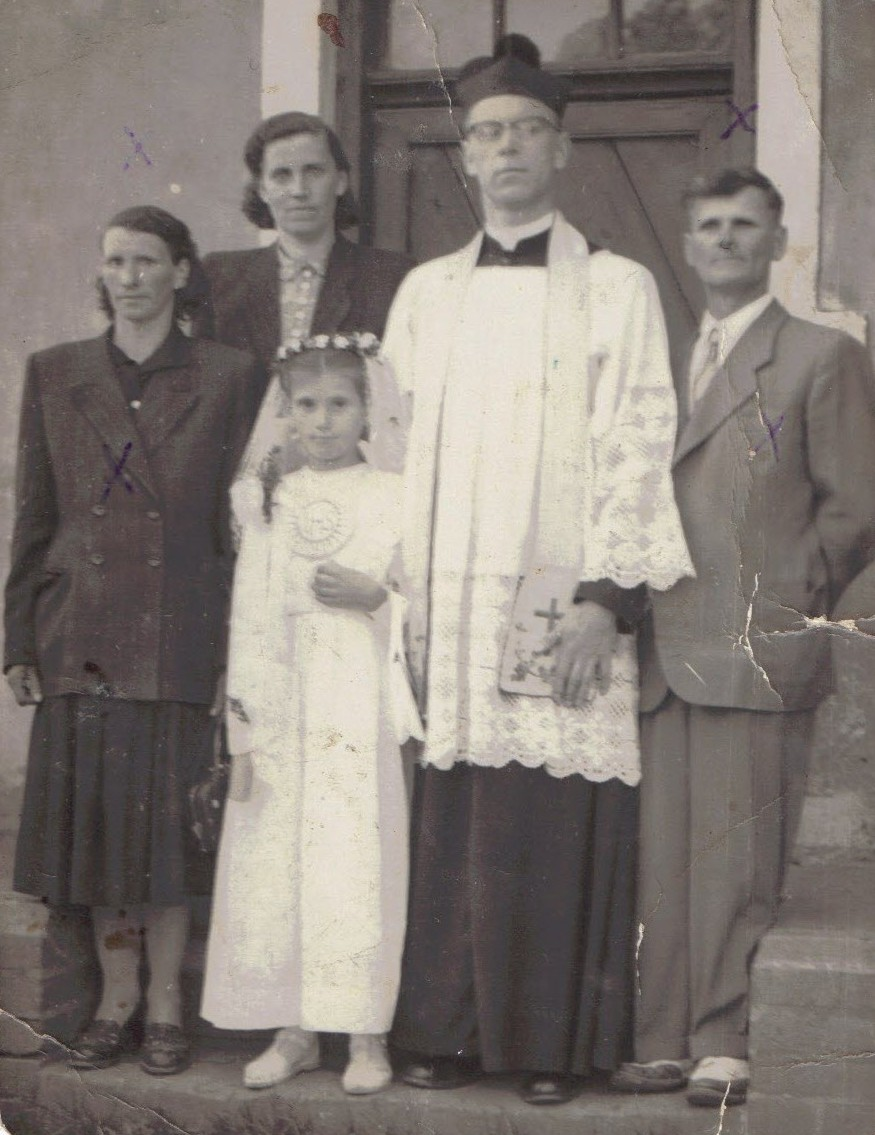
\includegraphics[width=0.45\textwidth]{zdjecia/pierwsza_komunia_miroslawy_glab.jpg}
\caption[Pierwsza Komunia św. Mirosławy Głąbianki]{Pierwsza komunia św. Mirosławy Głąbianki -- córki Franciszka. Od lewej stoją: mama Eleonora Głąb z domu Merta, powyżej matka chrzestna Stanisława Merta (żona brata -- Mariana Merty), obok ksiądz Jan Merta (brat Eleonory) i ojciec Franciszek Głąb}
\label{rys:pierwsza_komunia_miroslawy_glab}
\end{center}
\end{figure}

\begin{figure}
\begin{center}
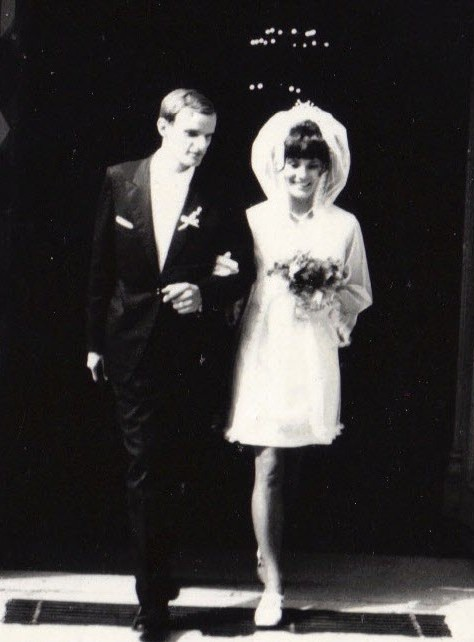
\includegraphics[width=0.4\textwidth]{zdjecia/slub_jerzego_i_miroslawy_jablonskich.jpg}
\caption{Ślub Mirosławy Głąbianki z Jerzym Jabłońskim}
\label{rys:slub_jerzego_i_miroslawy_jablonskich}
\end{center}
\end{figure}

Najstarsza córka Mirosława podjęła naukę w Technikum Gastronomicznym w Cieszynie w latach 1962~--~1967, a następnie w Studium Nauczycielskim w Częstochowie, gdzie poznała swego wybrańca losu -- Jurka Jabłońskiego, niezwykle inteligentnego i wysportowanego studenta Politechniki Częstochowskiej.

%\begin{sidewaysfigure}
\begin{sidewaysfigure}	
\begin{center}
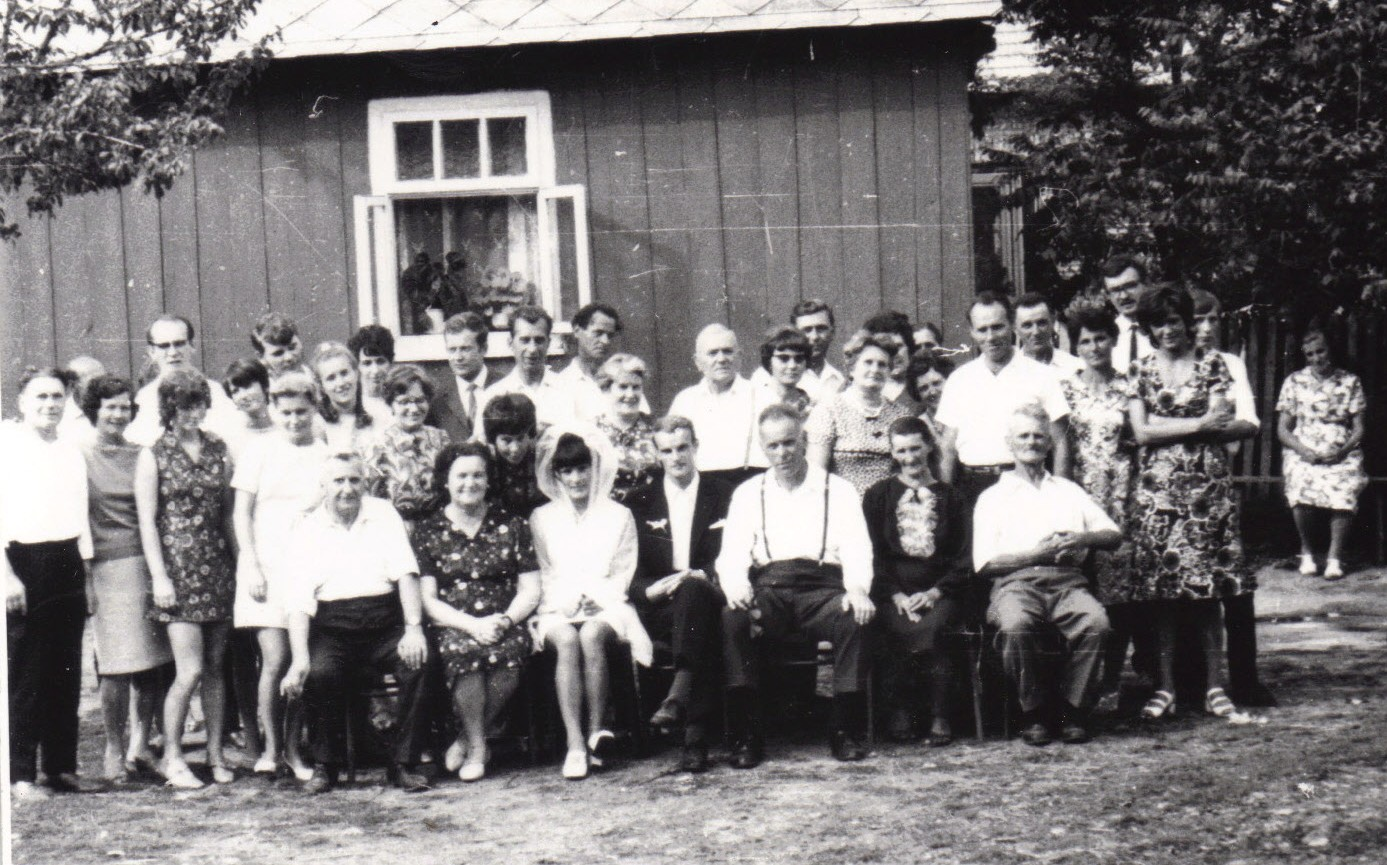
\includegraphics[height=130mm]{zdjecia/slub_jerzego_i_miroslawy_jablonskich_zbiorowe.jpg}
\caption[Zbiorowe zdjęcie ślubne Mirosławy i Jerzego Jabłońskich]{Zdjęcie ślubne Mirosławy Głąbianki i Jerzego Jabłońskiego. Od lewej siedzą: Wacław i Irena Jabłońscy (rodzice Jurka), Mira i Jerzy (Państwo Młodzi), ks. Jan Merta (brat Eleonory), Eleonora i Franciszek Głąbowie (rodzice Miry), od lewej stoją za siedzącymi: Stanisław Głąb z Anielą Głąb Biskupską (najmłodsi brat z siostrą Franciszka Głąba), Basia Głąbówna (najmłodsza siostra Miry), nieco za nią Czesia Głąbówna (młodsza siostra Miry), Ewa Stępień (z Warszawy), Anna Bienia, Iza Kusztal (z Warszawy), Czesława Jabłońska (z Lublina), Jadwiga Stępień (matka Ewy z Warszawy), Wacek Bubel, Irena Kusztal (mama Izy z Warszawy), Alfreda Głąb -- żona Stanisława -- ojca chrzestnego Miry, osoba nierozpoznana, Maria Łakota, Urszula Skupin (późn. żona Tomasza Świerczyńskiego), nieco za nią Mirek Głąb (brat Miry), w ostatnim rzędzie stoją od lewej: Andrzej Brożyna, Jan Bienia, Henia Świderska (z domu Zych), jej mąż, Wiesław Jabłoński (stryj Jurka), Marian Merta, za Wackiem Bublem stoją Zosia i Stach Karoniowie, zasłonięta Eleonora Bubel, Stanisław Łakota i Czesław Świerczyński.}
\label{rys:slub_jerzego_i_miroslawy_jablonskich_zbiorowe}
\end{center}
\end{sidewaysfigure}

Ukoronowaniem tej znajomości był ślub Mirosławy Głąbianki z Jerzym Jabłońskim (ur. 10 IX 1944~r. w Stalowej Woli z ojca Wacława i matki Ireny z domu Żelichowska), który się odbył w Niegowie 21 sierpnia 1971~r. Mają jedynego syna Rafała (ur. 7 XII 1972~r. w Rzeszowie) (ryc.~\ref{rys:slub_jerzego_i_miroslawy_jablonskich} i ~\ref{rys:slub_jerzego_i_miroslawy_jablonskich_zbiorowe}).

Jerzy Jabłoński po ukończeniu studiów na Politechnice Częstochowskiej, która wówczas była szanowaną uczelnią ze względu na wybitną kadrę naukową, w dużej części pochodzącą z uczelni lwowskich, zatrudnił się na Politechnice Rzeszowskiej, na stanowisku asystenta. Na tejże uczelni obronił pracę doktorską na temat nagniatania oscylacyjnego. 

W tym samym roku Mirosława Jabłońska ukończyła studia z tytułem magistra na Akademii Rolniczej w Poznaniu na Wydziale Technologii Żywności. Pracowała później jako nauczyciel zawodu najpierw w Iwoniczu Zdroju (w latach 1969 – 1971) a następnie w Zespole Szkół Gospodarczych w Rzeszowie (w latach 1971 – 2007). 

Jerzy Jabłoński w latach 2003 -- 2009 pracował jako adiunkt na Uniwersytecie Rzeszowskim, kiedy go dopadł nowotwór układu krwiotwórczego zwany szpiczakiem. Walczyli z nim wspólnie: ojciec Jerzy z synem Rafałem, który dzięki swej determinacji i możliwościom zawodowym znalazł ojcu najlepsze miejsce -- w Klinice Lubelskiej, specjalistów i środki do walki z tą odmianą raka. Mimo tych wyjątkowych zmagań Jurek Jabłoński zmarł 21 lipca 2009~r. w Rzeszowie. Przed odejściem jednak wykazał się ogromną wolą życia.
%TODO sprawdzić!!!
Oto na 5 dni przed śmiercią wziął udział w turnieju szachowym o tytuł Mistrza Miasta Rzeszowa (na który dotarł rowerem) i go wygrał. Data 21 (oczko) wystąpiła w jego życiu w ważnych momentach: ślub, obrona pracy doktorskiej i śmierć.

Rafał Jabłoński ukończył studia farmaceutyczne w Poznaniu i pracuje w NFZ w Rzeszowie. Ożenił się 30 IV 2000~r. w Rzeszowie w par. katedralnej z Agnieszką Hoszowską ur. 12 VI 1970r. w Rzeszowie z ojca Stanisława i matki Anny z domu Pielech (ryc.~\ref{rys:slub_rafala_i_agnieszki_jablonskich}).

\begin{figure}
\begin{center}
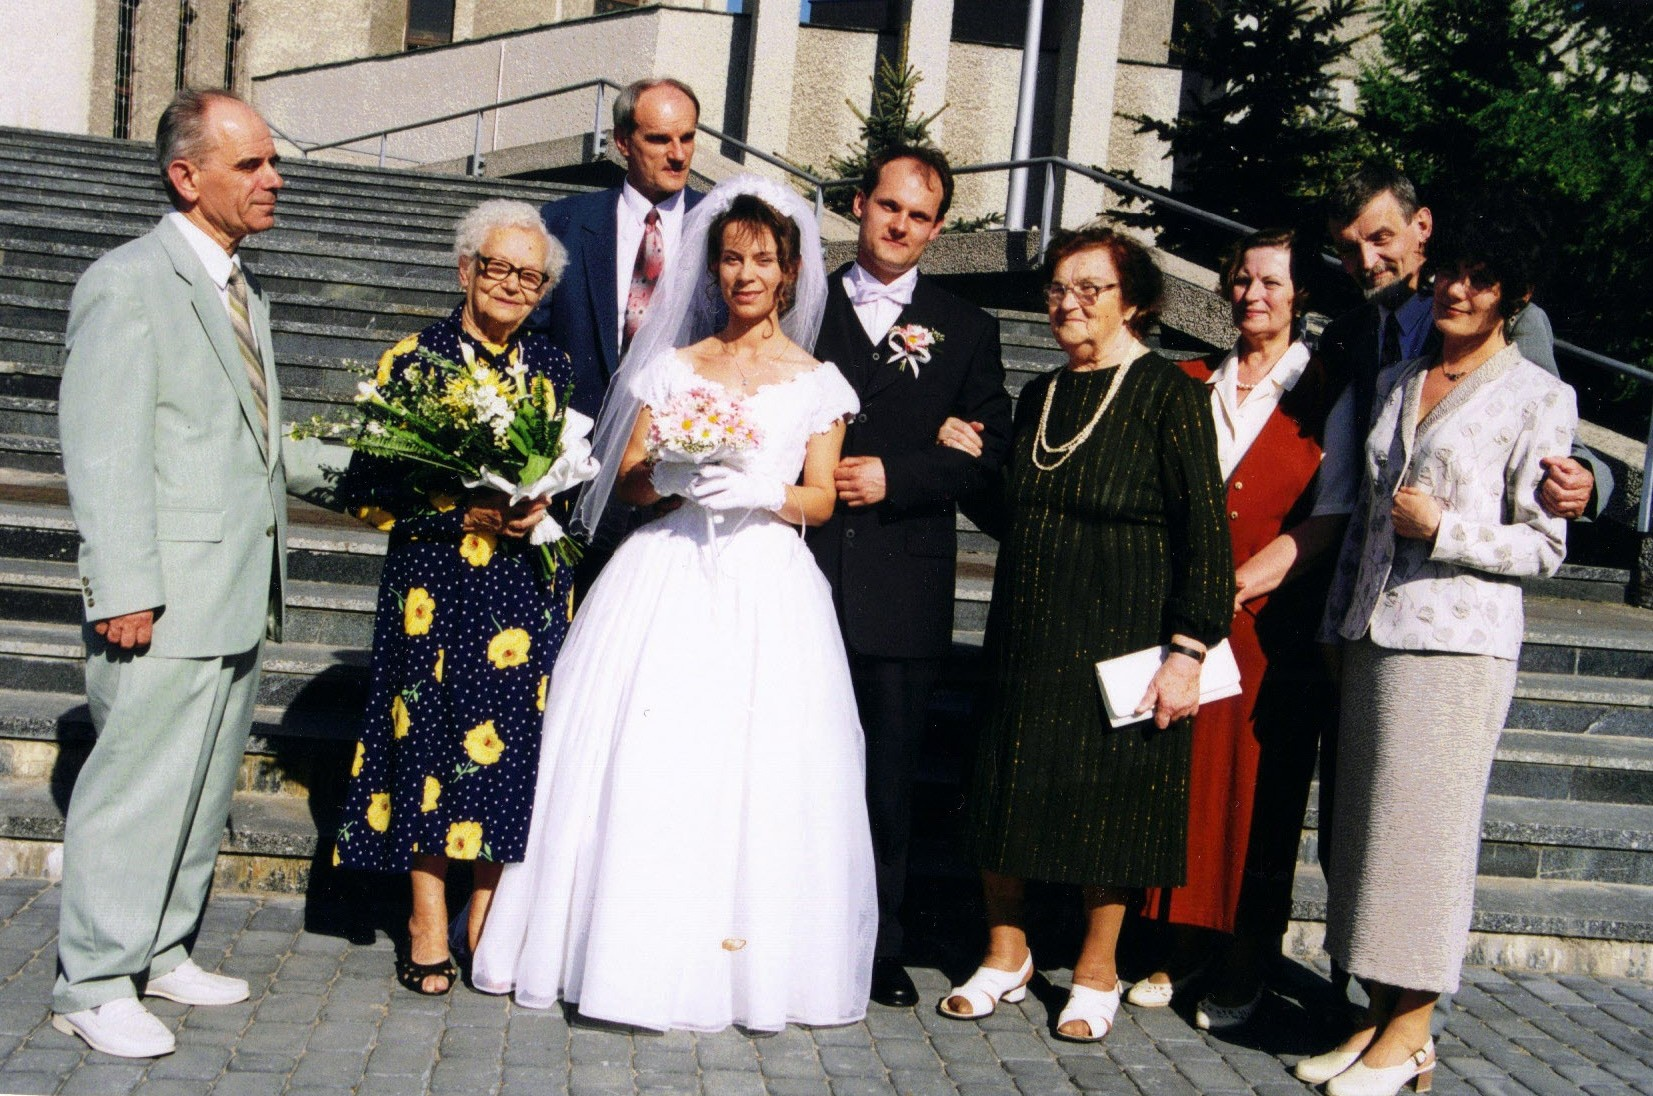
\includegraphics[width=0.7\textwidth]{zdjecia/slub_rafala_i_agnieszki_jablonskich.jpg}
\caption[Ślub Agnieszki Hoszowskiej z Rafałem Jabłońskim]{Ślub Agnieszki Hoszowskiej i Rafała Jabłońskiego. Na zdjęciu od lewej stoją: Stanisław Hoszowski (ojciec Agnieszki), Maria Pielech (babcia Pani Młodej), z tyłu Jerzy Jabłoński (ojciec Rafała), Agnieszka i Rafał Jabłońscy, babcia Rafała -- Irena z Żelichowskich Jabłońska, Krystyna Bula (chrzestna Rafała), Czesław Świerczyński (chrzestny Rafała) oraz Mira Jabłońska (mama Rafała)}
\label{rys:slub_rafala_i_agnieszki_jablonskich}
\end{center}
\end{figure}

\begin{figure}
\begin{center}
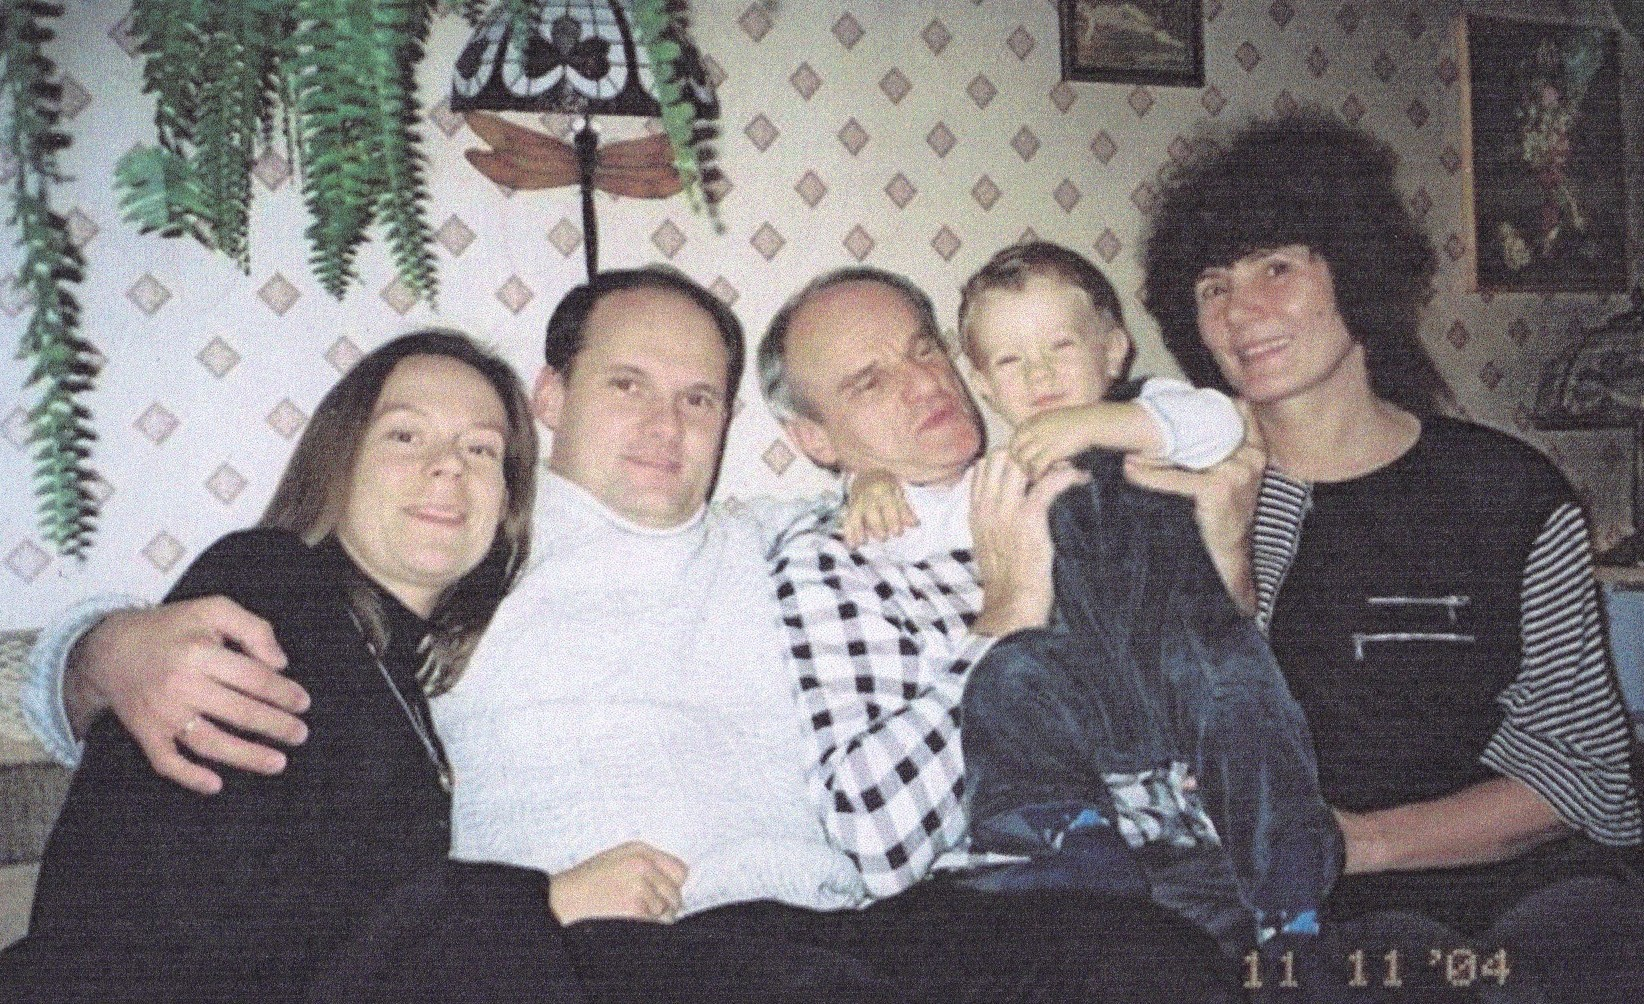
\includegraphics[width=0.8\textwidth]{zdjecia/jedrek_jakblonski_i_rodzina.jpg}
\caption[Jędrek Jabłoński z rodzicami i dziadkami]{Jędrek Jabłoński z rodzicami i dziadkami. Od lewej: Agnieszka i Rafał Jabłońscy -- rodzice, dalej Jerzy i Mirosława Jabłońscy (dziadkowie)}
\label{rys:jedrek_jakblonski_i_rodzina}
\end{center}
\end{figure}


\begin{figure}
	\begin{center}
		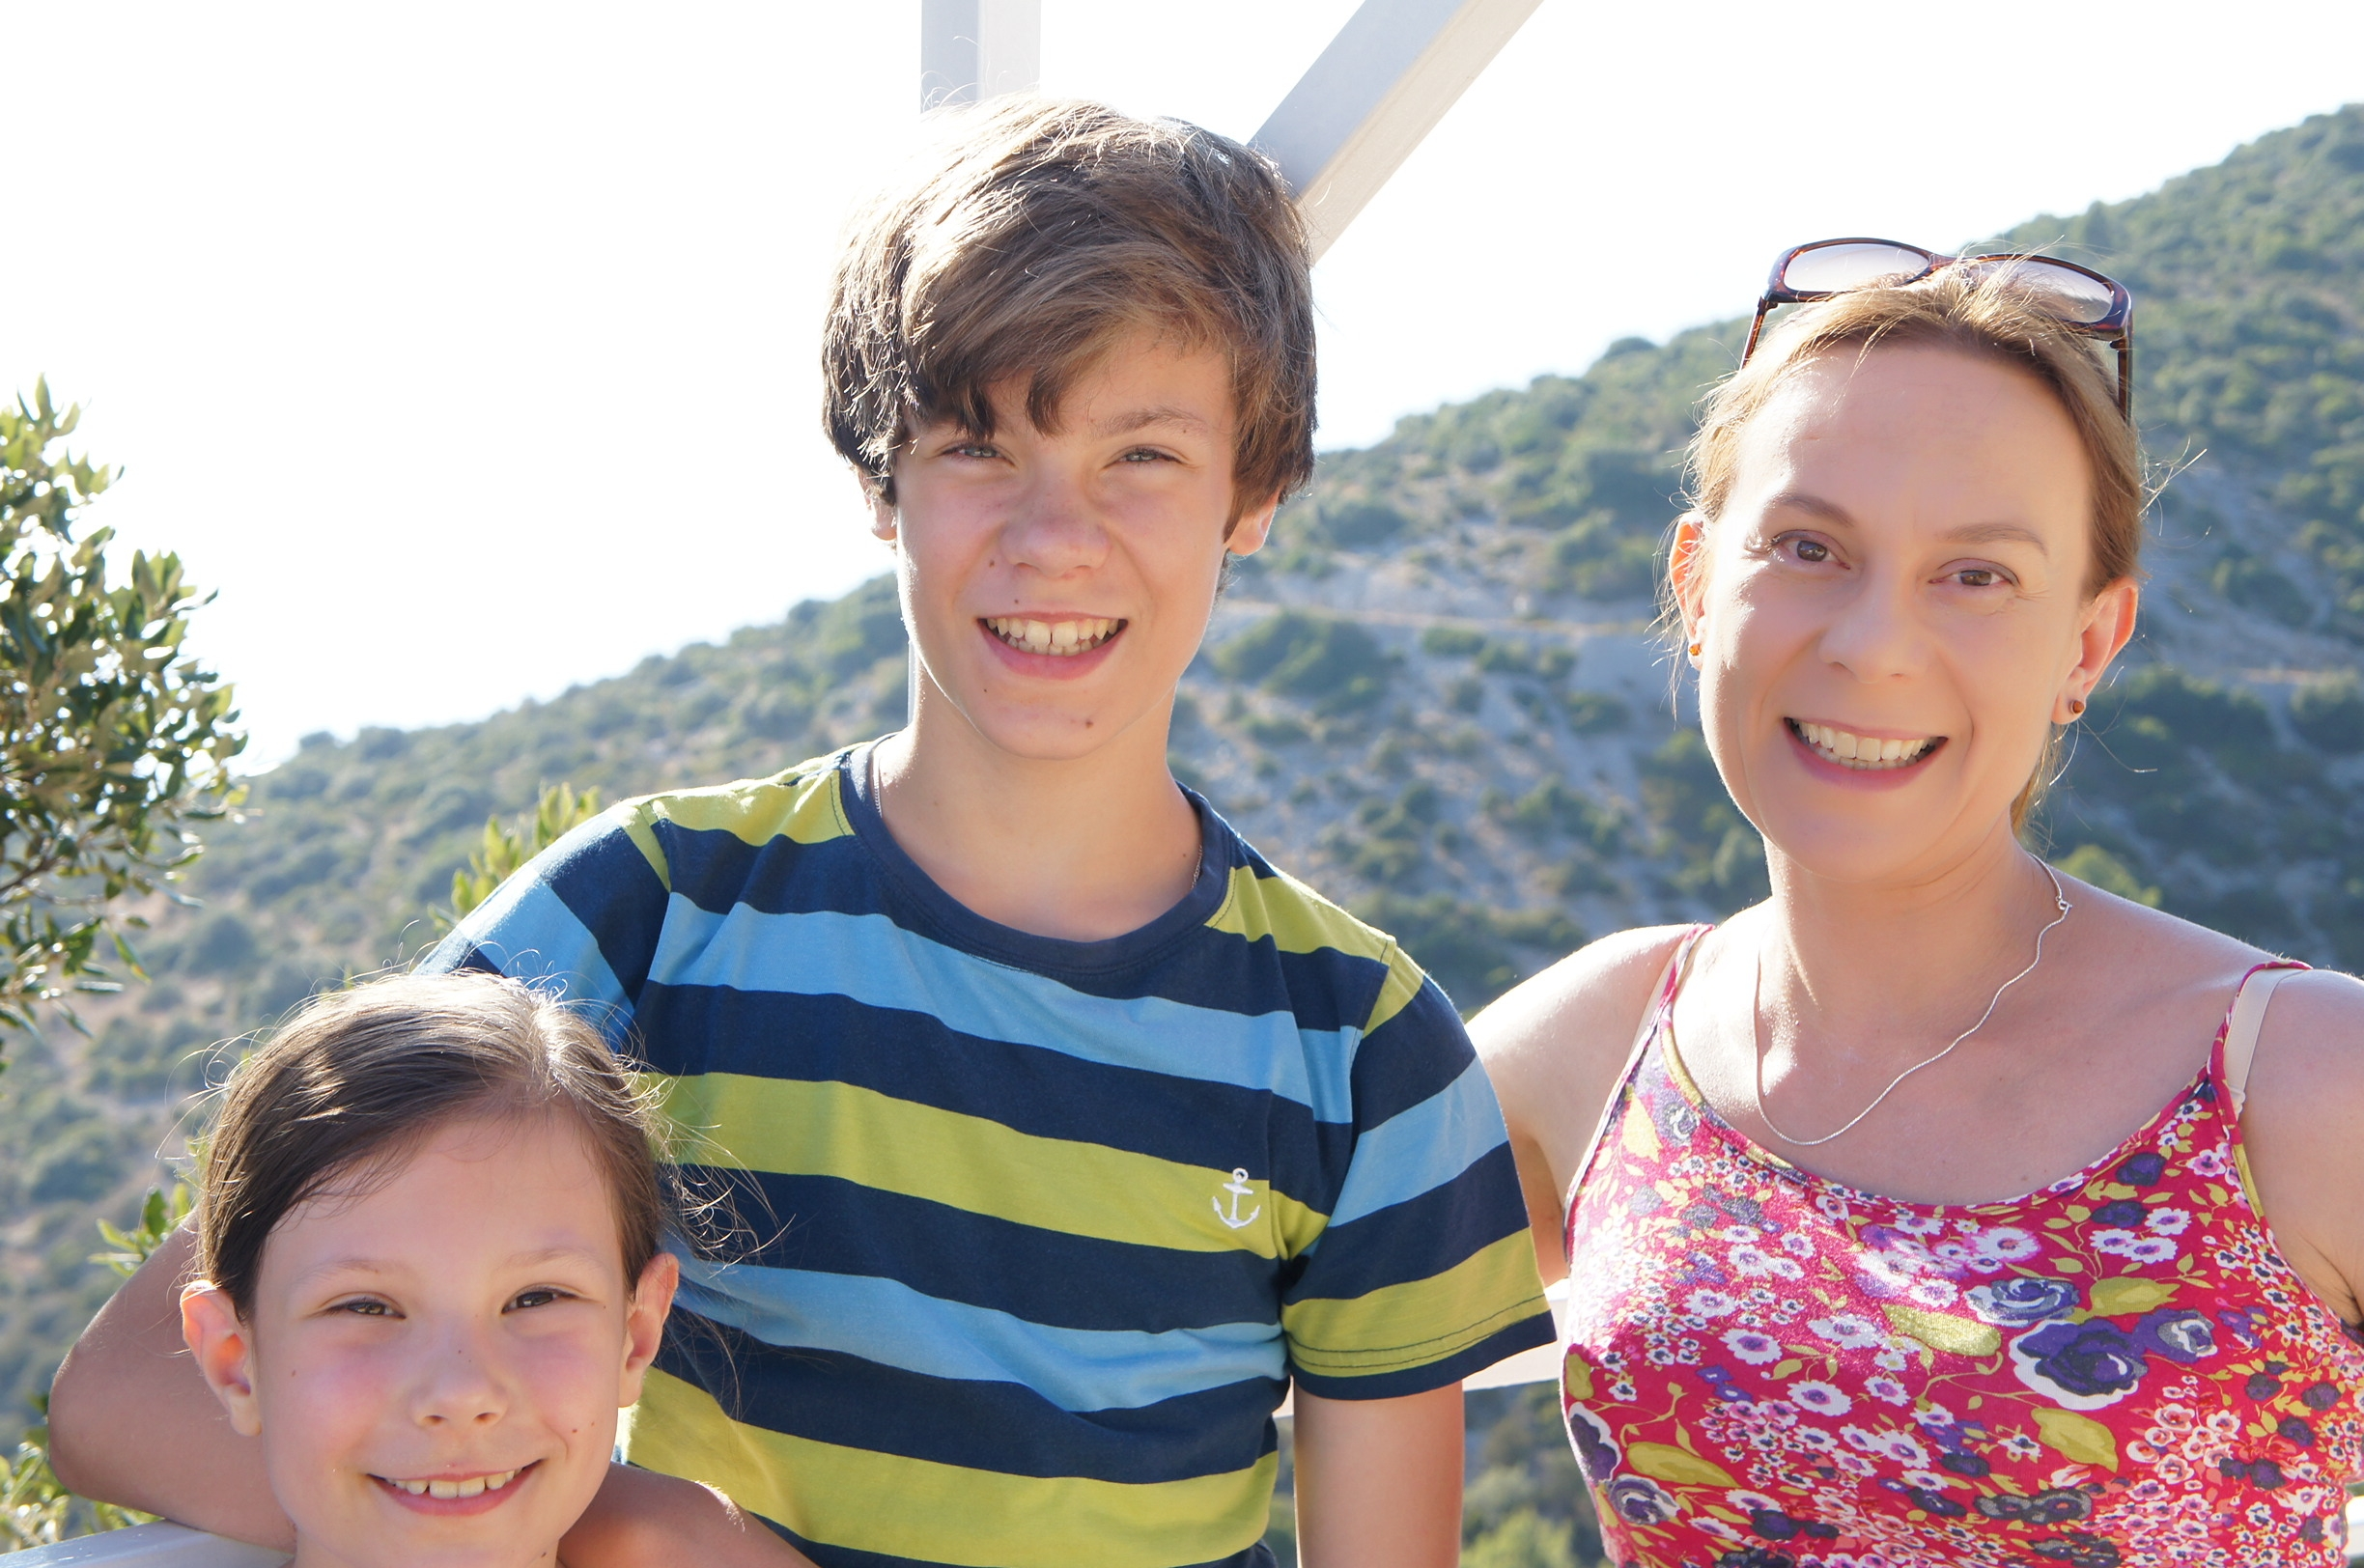
\includegraphics[width=0.8\textwidth]{zdjecia/agnieszka_jedrek_alicja_jablonscy.jpg}
		\caption{Agnieszka Jabłońska z synem Jędrkiem i córką Alicją}
		\label{rys:agnieszka_jedrek_alicja_jablonscy}
	\end{center}
\end{figure}

\begin{figure}
	\begin{center}
		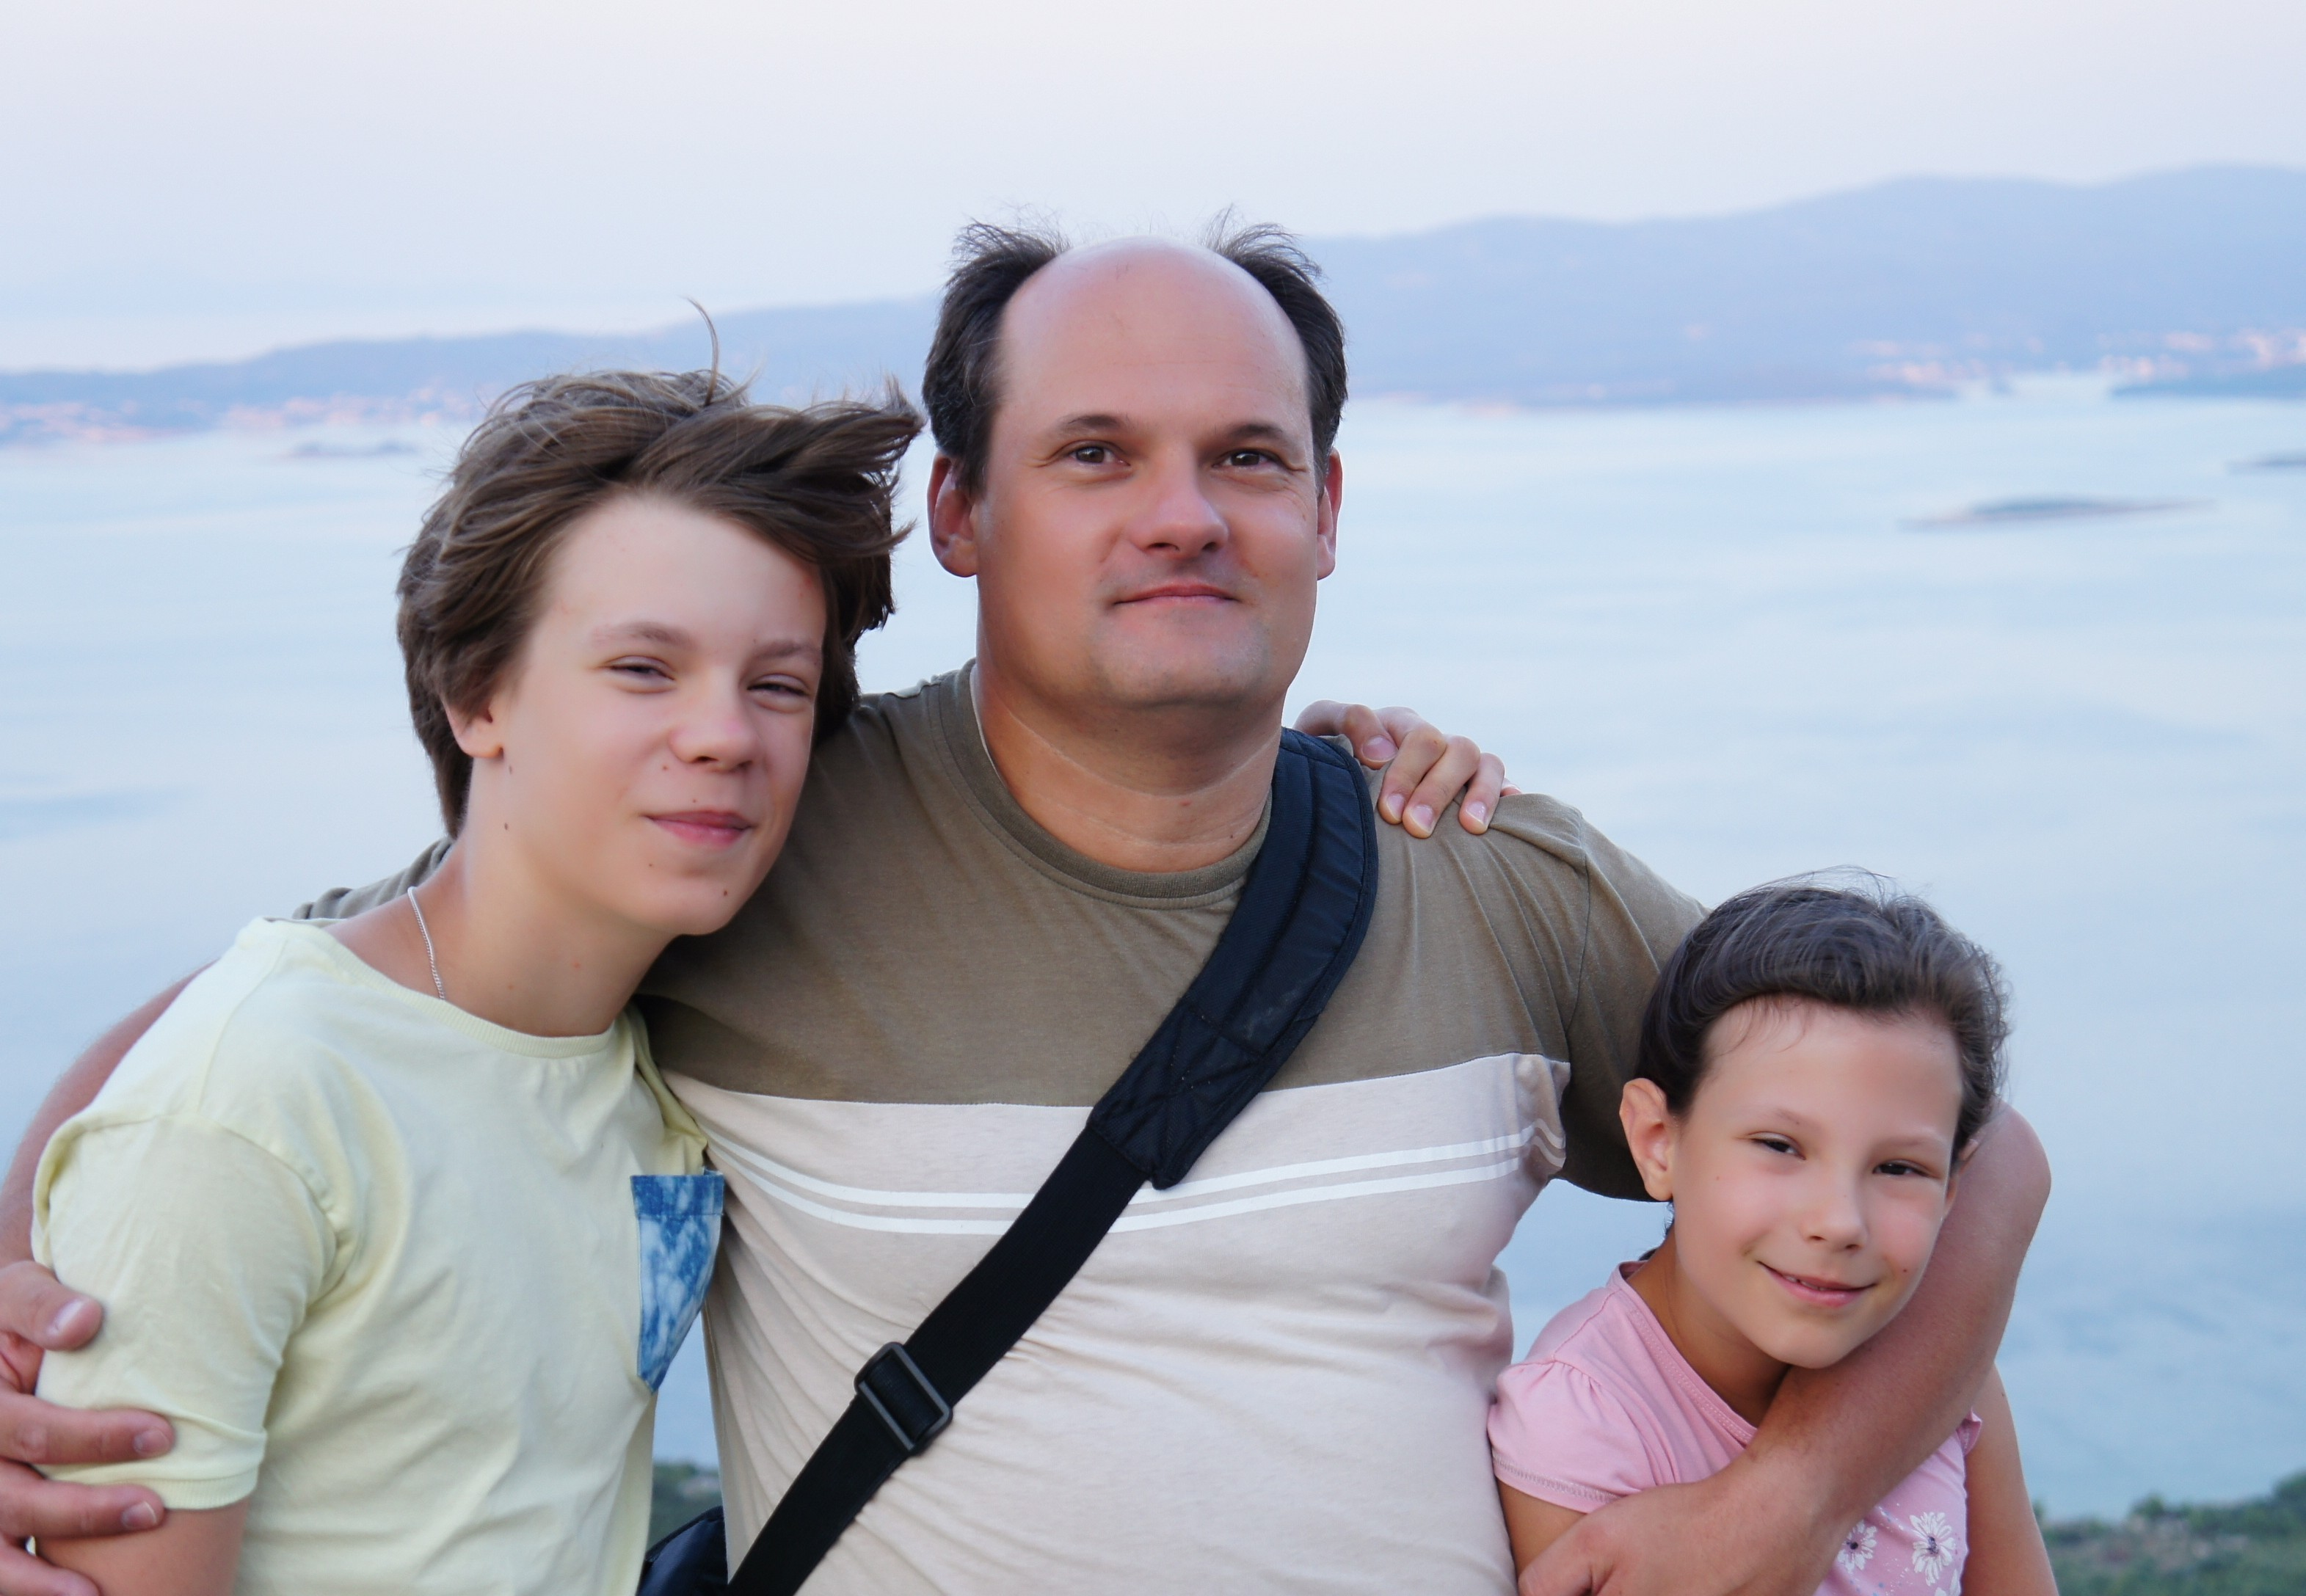
\includegraphics[width=0.8\textwidth]{zdjecia/rafal_jablonski_z_dziecmi.jpg}
		\caption{Rafał Jabłoński z córką Alicją i synem Jędrkiem}
		\label{rys:rafal_jablonski_z_dziecmi}
	\end{center}
\end{figure}




Jego małżonka jest doktorem w Instytucie Muzyki Uniwersytetu Rzeszowskiego w Zakładzie Gry Fortepianowej.  Doczekali się dwójki dzieci: syna Andrzeja ur. 12 III 2003~r. w Kolbuszowie oraz Alicji ur. 16 V 2007~r. w Rzeszowie (ryc.~\ref{rys:jedrek_jakblonski_i_rodzina}, \ref{rys:agnieszka_jedrek_alicja_jablonscy} i \ref{rys:rafal_jablonski_z_dziecmi}). Jędrek jest uczniem Szkoły Muzycznej w Rzeszowie i kilkukrotnym laureatem konkursów pianistycznych.





\section{Czesława Świerczyńska z domu Głąb}

\begin{figure}
\begin{center}
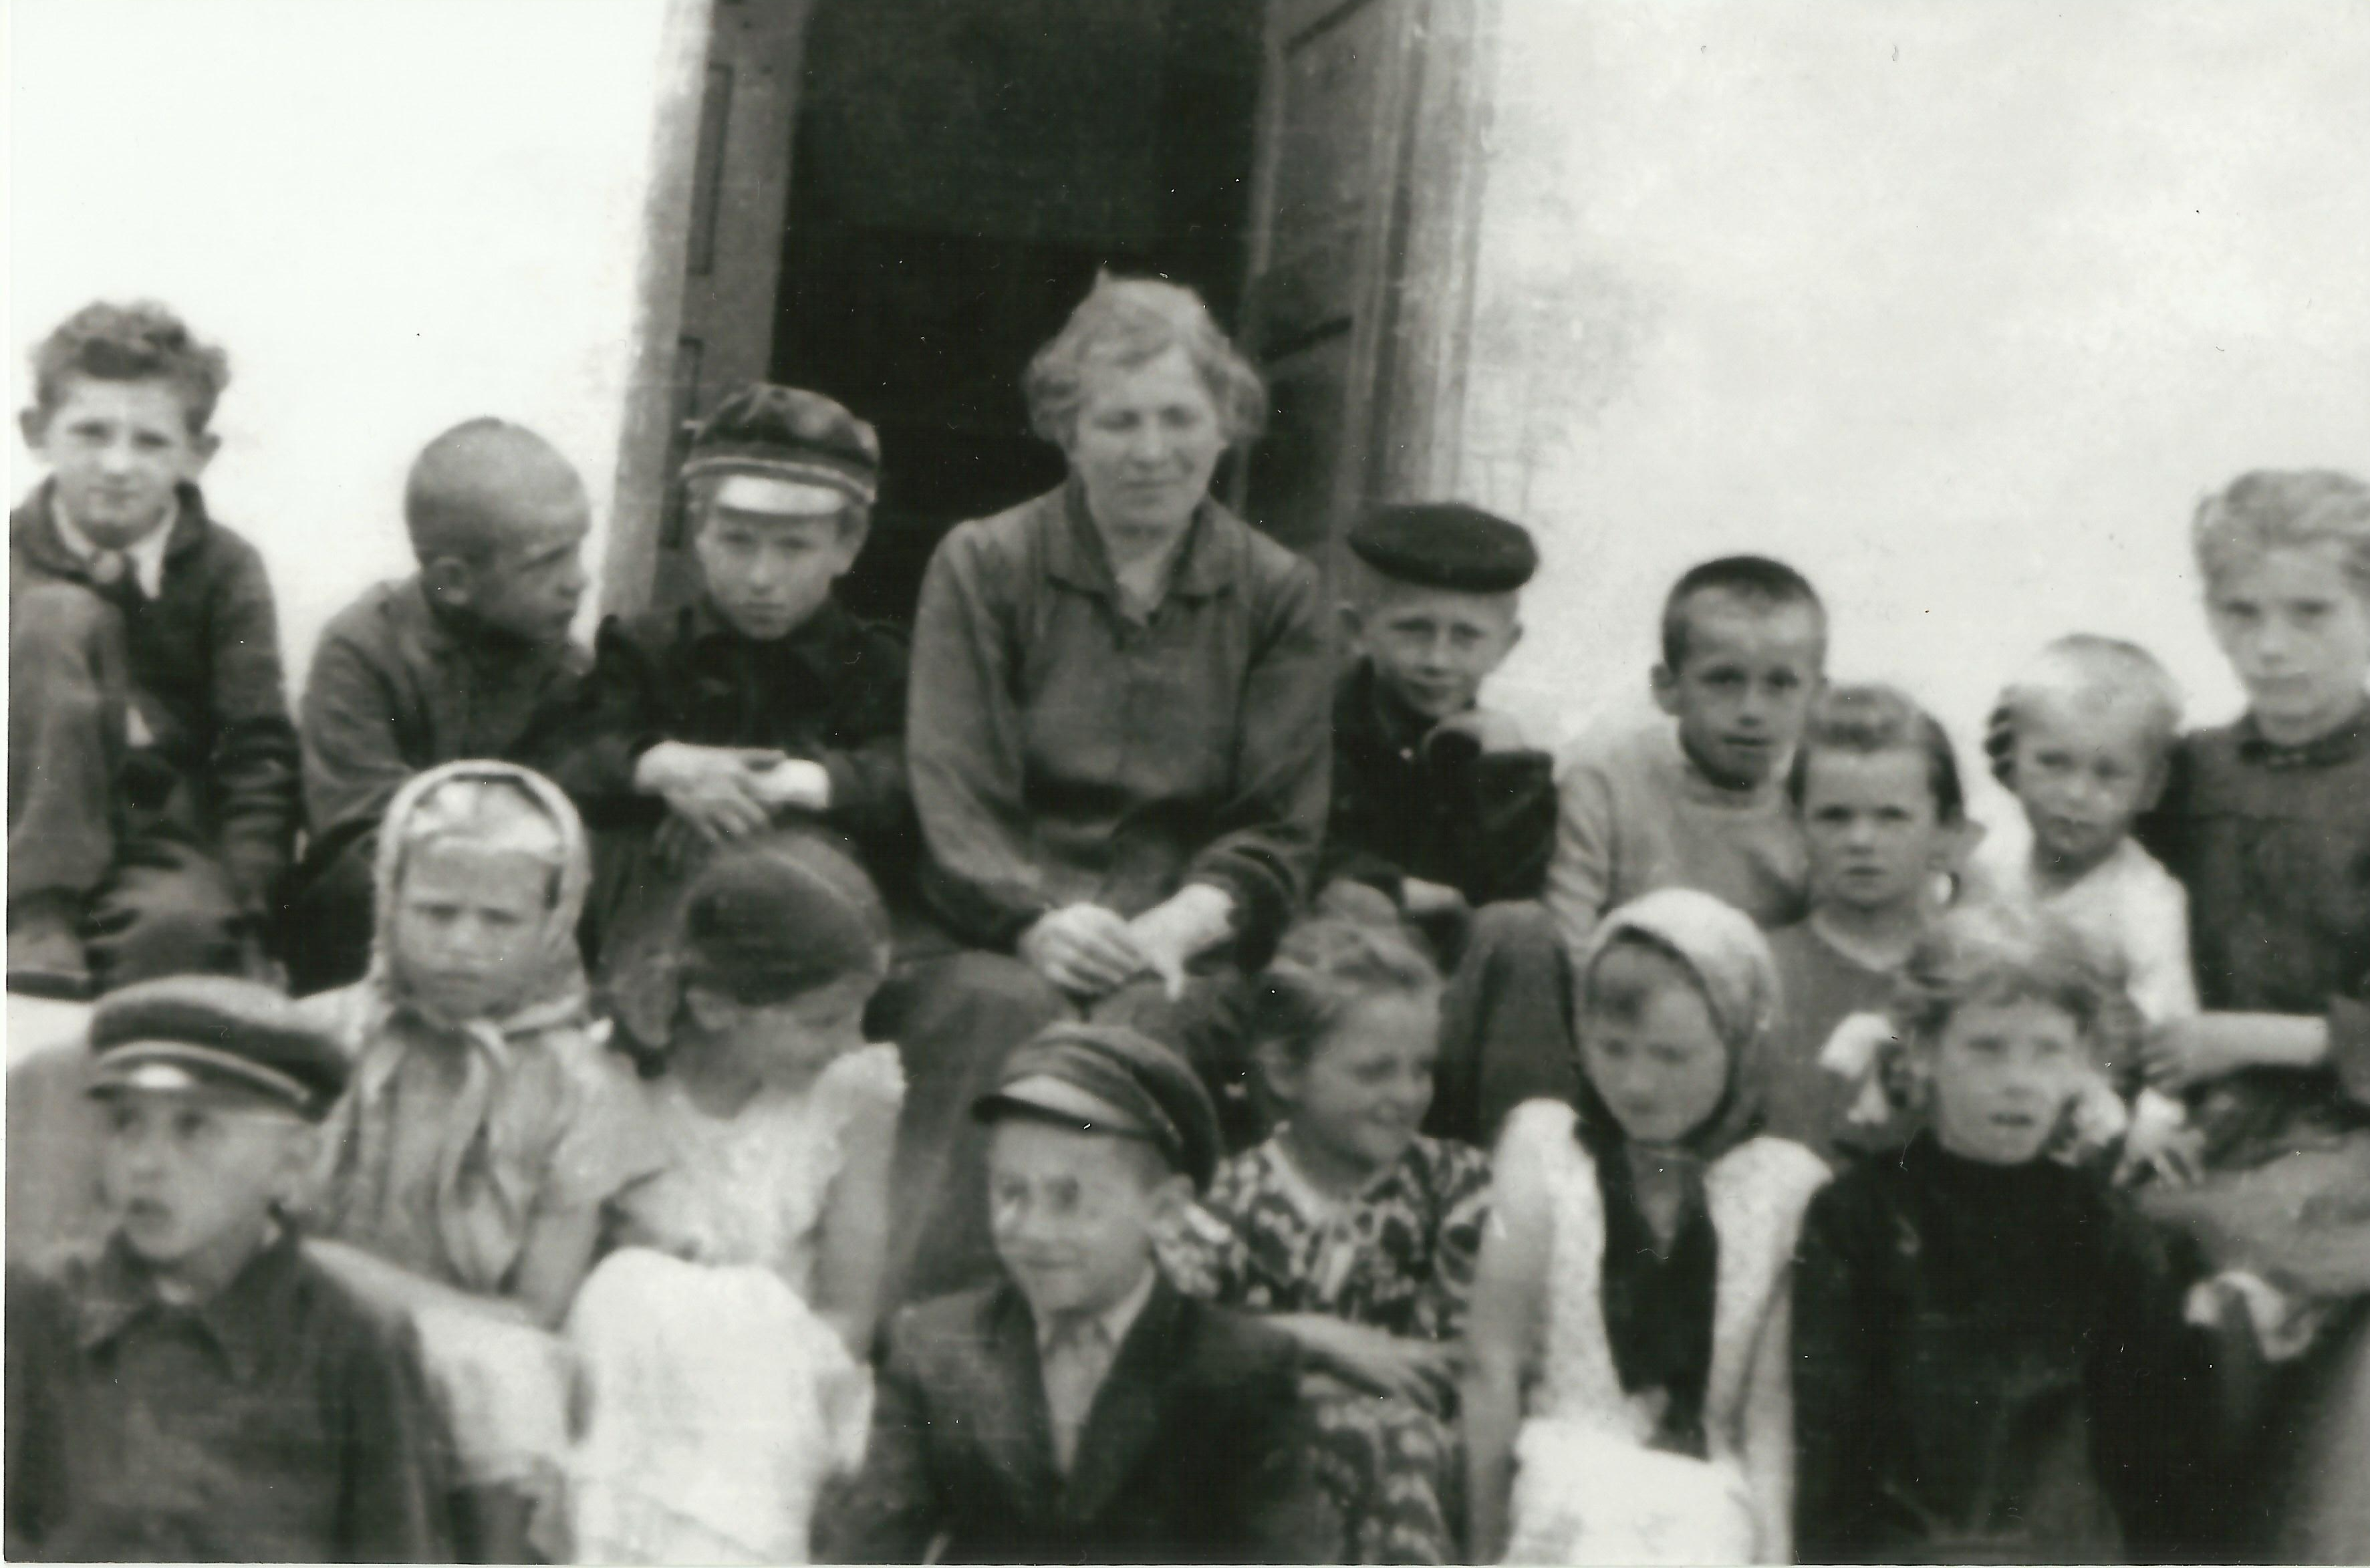
\includegraphics[width=\textwidth]{zdjecia/szkola_w_mirowie.jpg}
\caption[Uczniowie Szkoły Podstawowej w Mirowie]{Uczniowie Szkoły Podstawowej w Mirowie ze swoją nauczycielką. Od lewej w dolnym rzędzie: Stanisław Radosz, Marta Męcik, Stanisława Męcik, Stanisław Tylkowski, Genowefa Mucha, Anna Ślęzak, Czesława Głąb, w górnym rzędzie od lewej: Zenon Męcik, Jan Gurbała, Stanisław Baryła, nauczycielka Irena Wesołowska, Walenty Grzegorz Kurek, Stanisław Hamerla, Maria Gradzik, Mirosław Głąb, Mirosława Głąbianka.}
\label{rys:szkola_w_mirowie}
\end{center}
\end{figure}

\begin{sidewaysfigure}
	\begin{center}
		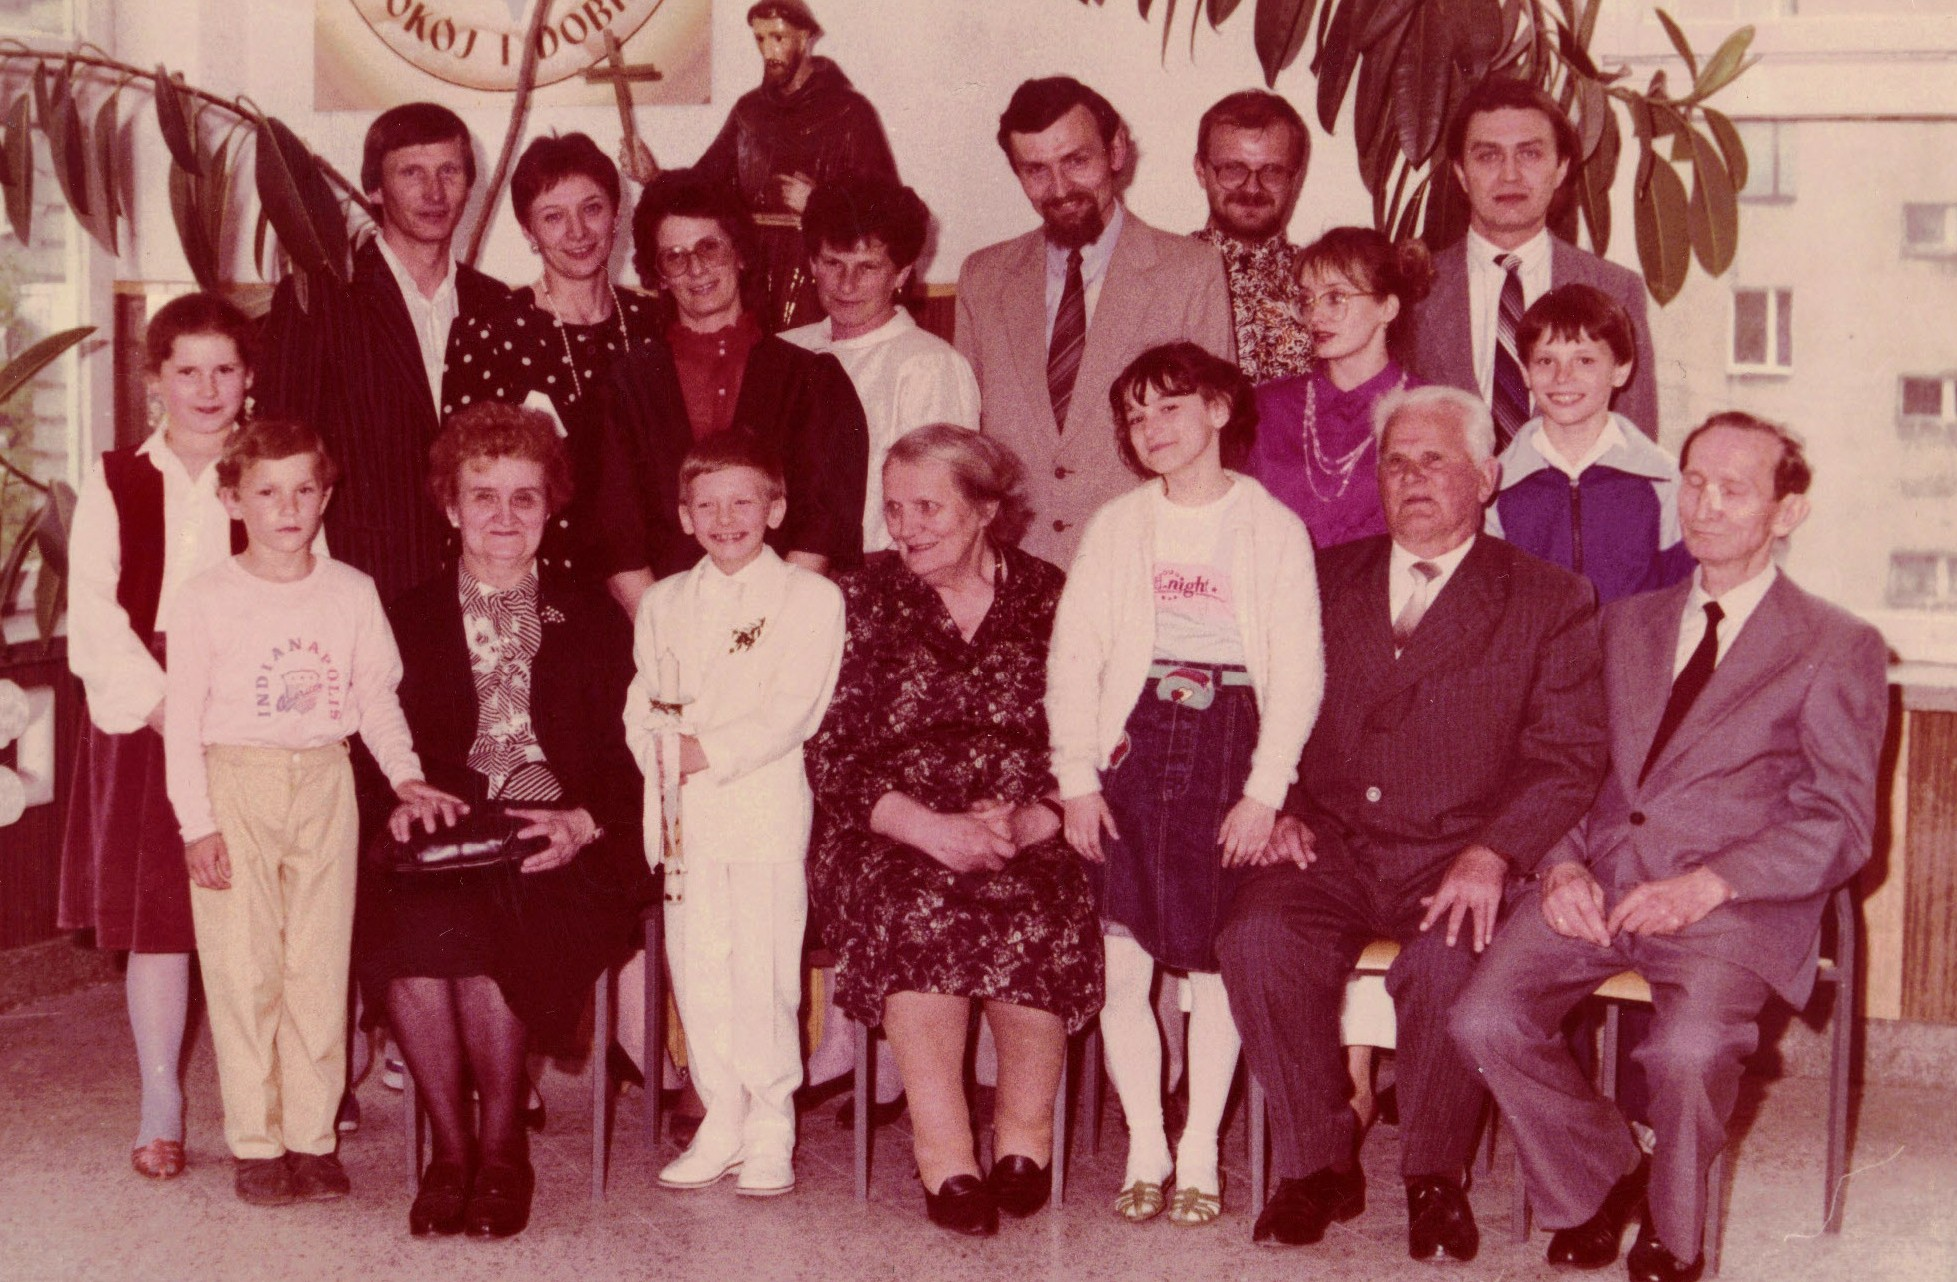
\includegraphics[height=150mm]{zdjecia/komunia_bozydara_swierczynskiego_zbiorowe.jpg}
		\caption[Pierwsza Komunia św. Bożydara Świerczyńskiego -- zdjęcie zbiorowe]{Pierwsza Komunia św. Bożydara Świerczyńskiego: na zdj. od lewej w I rzędzie: Kasia i Irek Wilk (dzieci Barbary Wilk z domu Głąb), Radegunda Świerczyńska (babcia Bożydara), Bożydar, Irena Lehman (siostra dziadka Benedykta -- położna która przyjmowała Zuzię, Bożydara i Piotrusia), Agnieszka Głąbówna (córka Mirosława), dziadek Franciszek Głąb, dziadek Benedykt Świerczyński, w drugim rzędzie stoją od lewej: Mirosław Głąb (chrzestny), Zosia Prele (chrzestna), Czesława Świerczyńska (mama), Barbara Wilk (siostra Czesławy), Czesław Świerczyński (tato), Marek (wnuk Ireny) i Małgosia Lehmanowie, Tomasz Świerczyński (brat Czesława) i przed nim Miłosz Głąb -- syn Mirosława.}
		\label{rys:komunia_bozydara_swierczynskiego_zbiorowe}
	\end{center}
\end{sidewaysfigure}

Opodal domu rodzinnego Walentego i Antoniny Głąbów, (który odziedziczył po nich syn Franciszek) stał budynek szkoły podstawowej w Mirowie (dzisiaj remiza strażacka), do której uczęszczała cała ówczesna mirowska dzieciarnia, jaką widać na zdjęciu (ryc.~\ref{rys:szkola_w_mirowie}).

\begin{figure}
\begin{center}
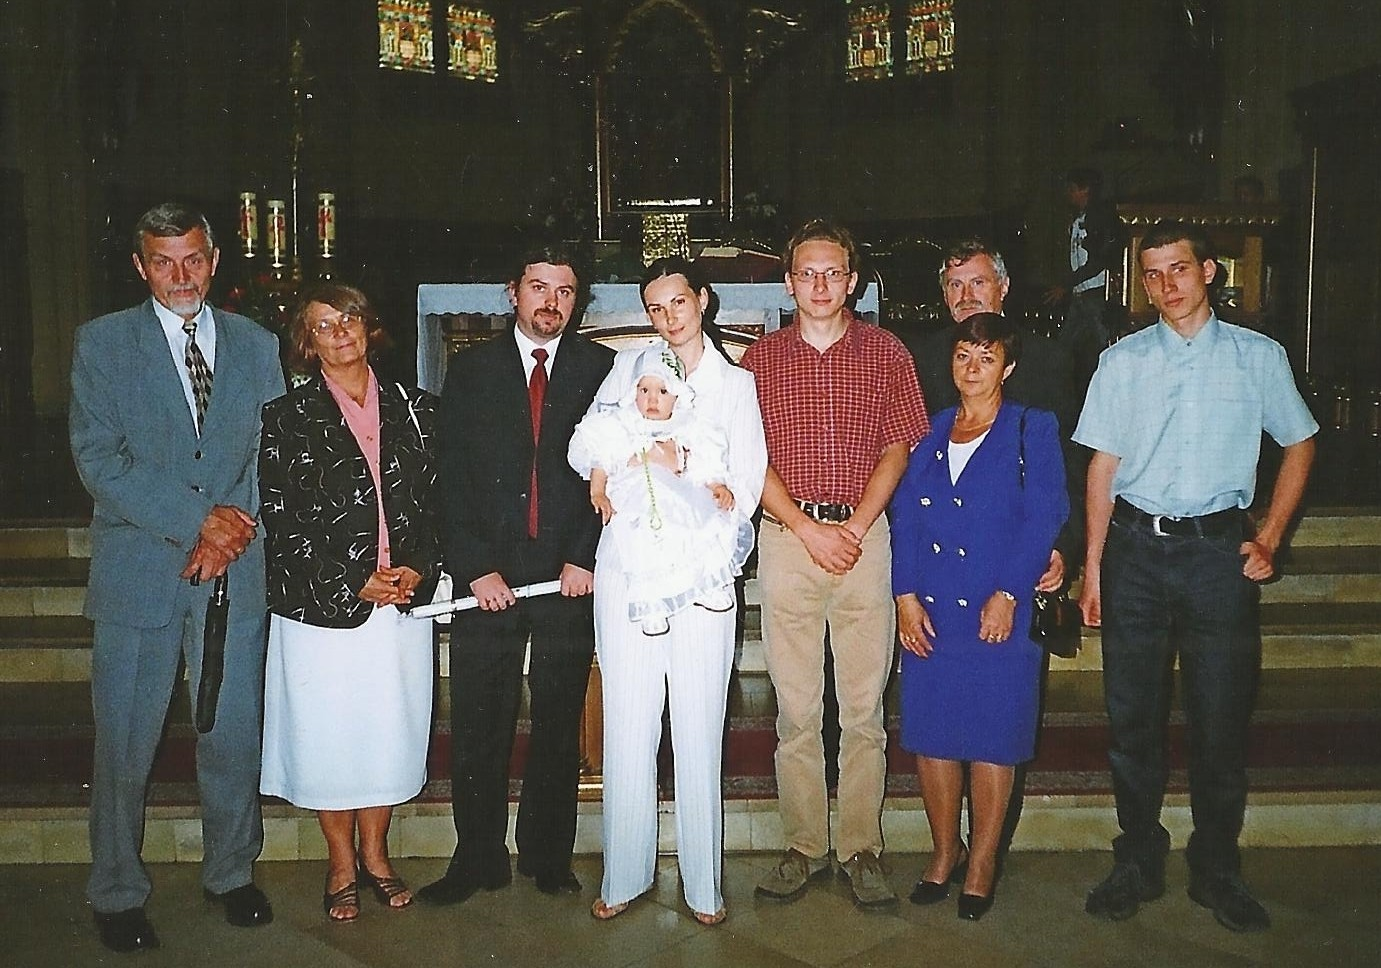
\includegraphics[width=0.8\textwidth]{zdjecia/roczek_malgorzaty_kordus.jpg}
\caption[Roczek Małgorzaty Kordus]{Roczek Małgosi Kordusównej w kościele św. Szczepana w Katowicach Bogucicach. Na zdjęciu od lewej: Czesław Świerczyński, Czesława Świerczyńska, Krzysiu Kordus, Zuzia ze Świerczyńskich Kordus, Bożydar Świerczyński, Wiesława i (z tyłu) Franciszek Kordusowie (rodzice Krzysia) oraz Piotr Świerczyński}
\label{rys:roczek_malgorzaty_kordus}
\end{center}
\end{figure}

Młodsza Czesława ukończyła studia polonistyczne na Uniwersytecie Śląskim. Na krótko przed jej zamążpójściem zmarła jej mama Eleonora (4 V 1972~r.), a jej pogrzeb był manifestacją wdzięczności Mirowian za jej dobroć. Nieśli jej trumnę na ramionach do samego kościoła w Niegowie, mimo że obok jechała pusta furmanka. Czesława wyszła dnia 27 sierpnia 1972~r.  w Katowicach w par. pw. św. Ap. Piotra i Pawła za Czesława Świerczyńskiego (ur. 16 IX 1946~r. w Katowicach z ojca Benedykta ur. 23 II 1920, zm. 19 VII 1999 i matki Radegundy ur. 26 X 1921, zm. 25 X 2002) i ma z nim trójkę dzieci: Zuzannę (ur. 18 II 1975~r. w Katowicach), Bożydara (ur. 13 maja 1982~r. w Katowicach) oraz Piotra (ur. w Katowicach 4 IV 1987~r.).

\begin{figure}
\begin{center}
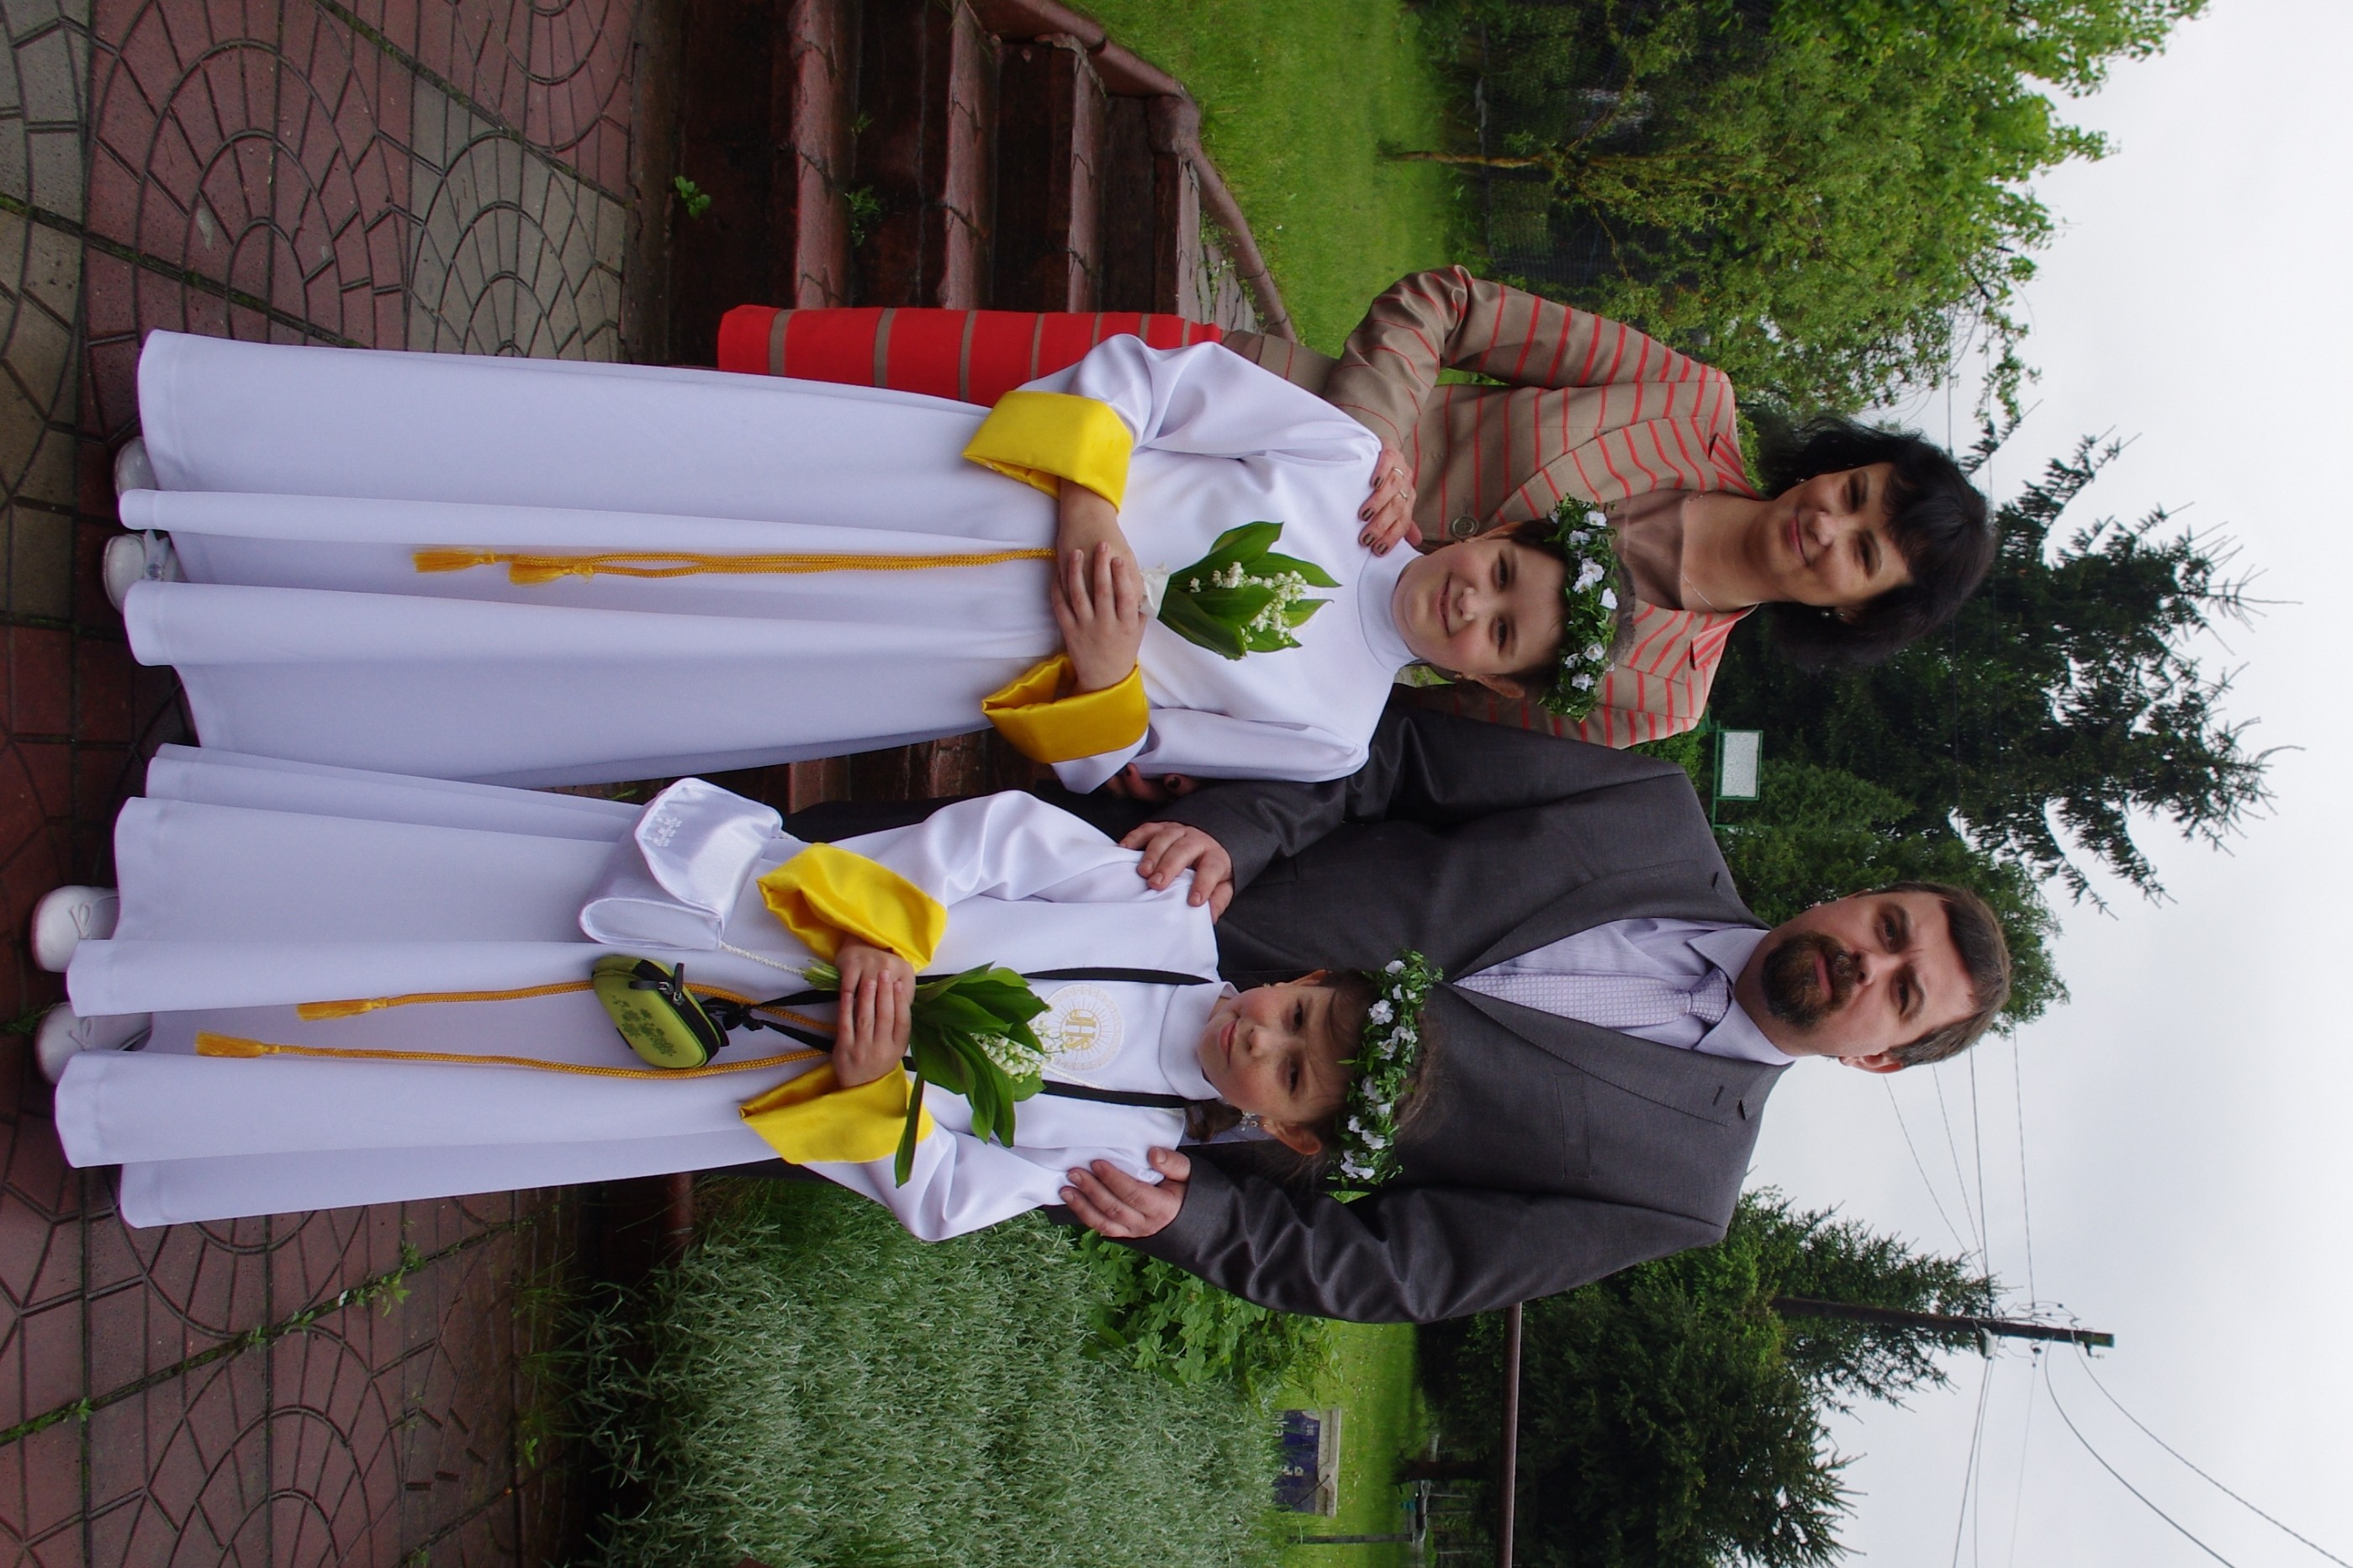
\includegraphics[width=0.5\textwidth, angle=90]{zdjecia/komunia_gosi_i_ani_kordus.jpg}
\caption[Pierwsza komunia św. Gosi i Ani Kordus]{Zdjęcie pierwszokomunijne Gosi i Ani Kordus wraz z rodzicami.}
\label{rys:komunia_gosi_i_ani_kordus}
\end{center}
\end{figure}

Wraz z dziećmi przez ponad 30 lat mieszkali w Myszkowie. Ich córka Zuzanna wyszła dnia 10 VIII 2002~r. za Krzysztofa Kordusa (ur. 20 IX 1976~r. w Katowicach z ojca Franciszka ur. 3 X 1953~r. i matki Wiesławy z Przybyszewskich ur. 12 V 1953 i niestety już zmarłej 12 II 2009 r.) i ma z nim dwie córki: Małgosię (ur. 11 VIII 2004~r. w Katowicach) (ryc.~\ref{rys:roczek_malgorzaty_kordus}) oraz Annę (ur. 7 IX 2006~r. w Katowicach) (ryc.~\ref{rys:komunia_gosi_i_ani_kordus}).

\begin{figure}[!h]
\begin{center}
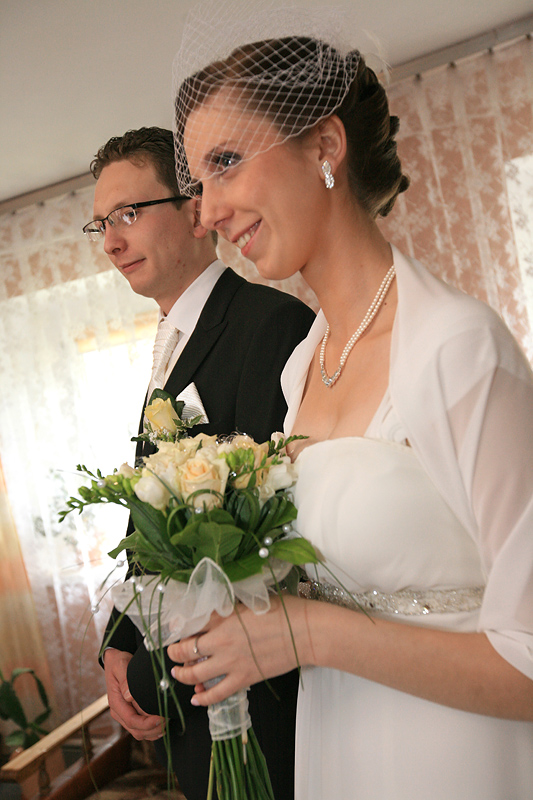
\includegraphics[width=0.4\textwidth]{zdjecia/slub_natalii_i_bozydara_swierczynskich.jpg}
\caption{Zdjęcie ślubne Natalii i Bożydara Świerczyńskich.}
\label{rys:slub_natalii_i_bozydara_swierczynskich}
\end{center}
\end{figure}

\begin{figure}[!hb]
\begin{center}
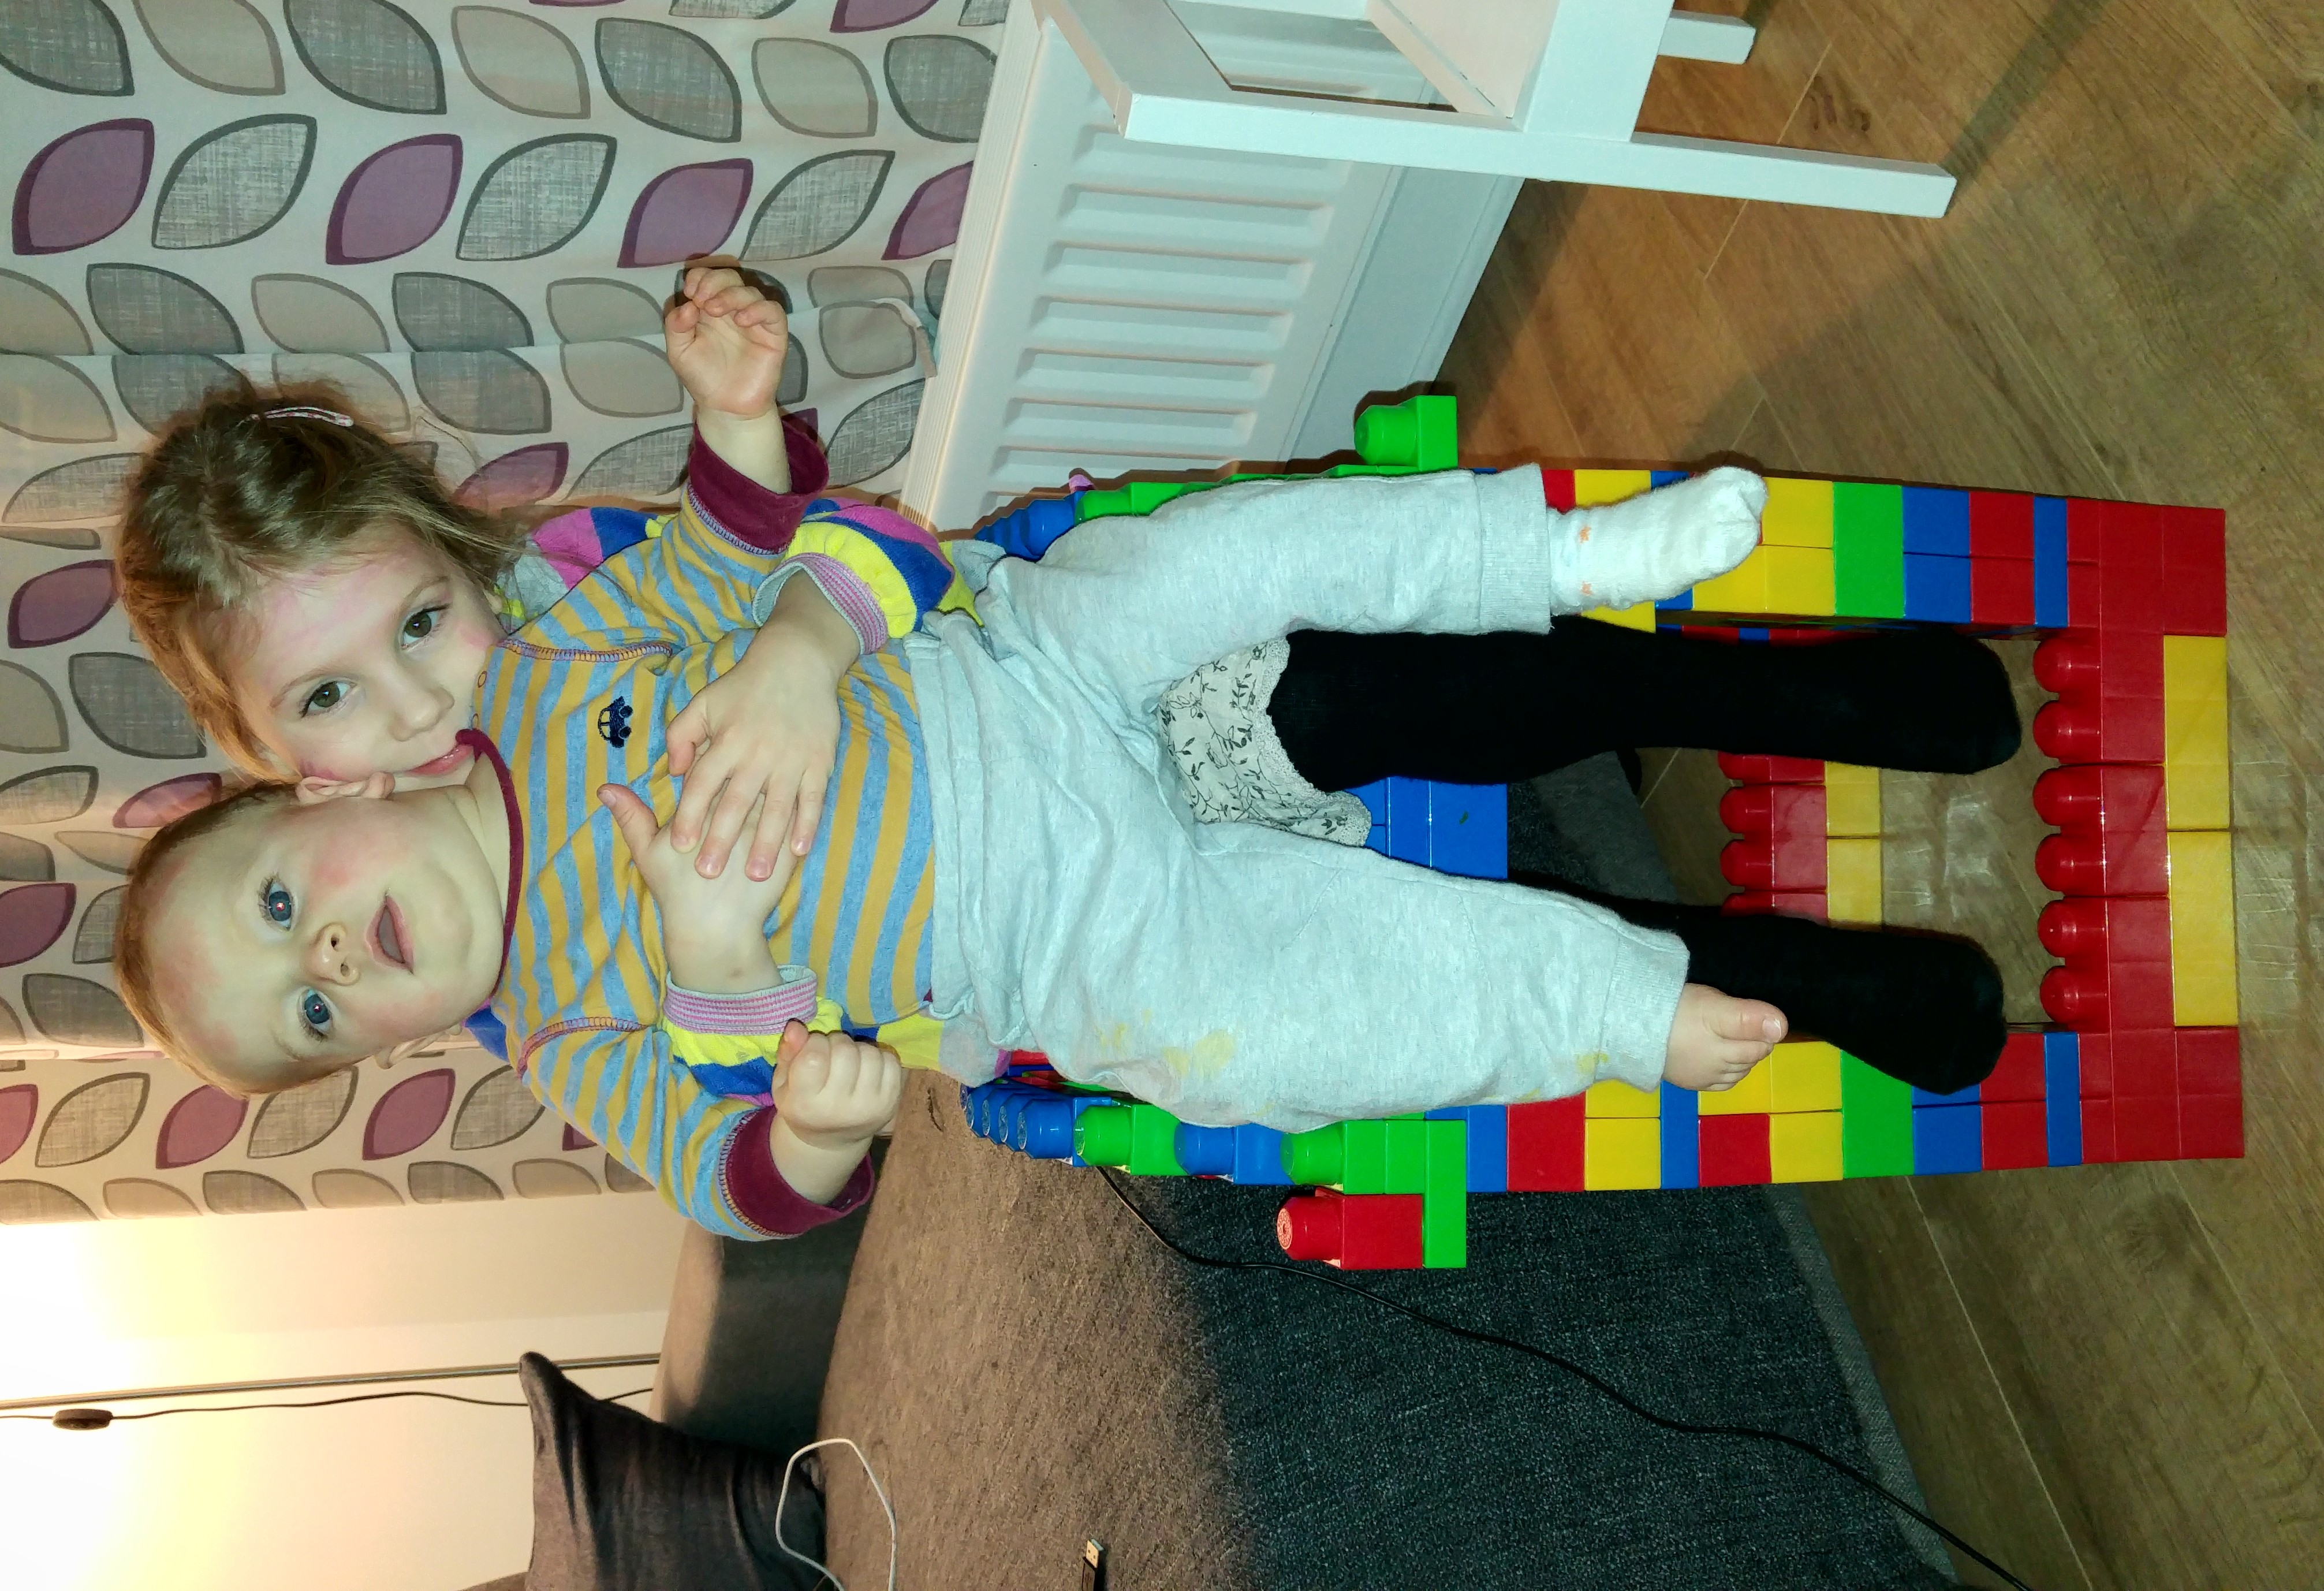
\includegraphics[width=0.6\textwidth, angle=270]{zdjecia/zofia_i_leon_swierczynscy.jpg}
\caption{Zofia i Leon Świerczyńscy.}
\label{rys:zofia_i_leon_swierczynscy}
\end{center}
\end{figure}

Bożydar ożenił się 4 września 2010~r. w Ziębicach z Natalią Gruszką (ur. 15 XII 1982~r. w Ziębicach z ojca Wiesława ur. 14 VI 1957~r. i matki Małgorzaty z Kluzów ur. 17 X 1961~r.) (ryc.~\ref{rys:slub_natalii_i_bozydara_swierczynskich}) i ma z nią córkę Zofię Helenę (ur. 30 I 2012~r. w Edynburgu, stolicy Szkocji) i syna Leona Michała (ur. 26 IV 2015~r., również w Edynburgu) (ryc.~\ref{rys:zofia_i_leon_swierczynscy}).


Piotr ożenił się 30 kwietnia 2011~r. w Kielcach z Justyną Sobczykówną (ur. 3 IX 1987~r. w Kielcach z ojca Sławomira ur. 4 VIII 1954 i matki Anny z Murczyńskich ur. 8 VII 1960), a ślubu udzielał im w katedrze bp Kazimierz Ryczan.

%TODO ***Tu zdj. ślubne Piotra i Justyny Świerczyńskich, jeśli takim dysponujesz lub zdj. Justyny Sobczyk z Anią Kordusówną. lub przynajmniej Jasiu zDziadkami Sobczykami
%TODO ***Tu zdj. Justyny na rękach Piotra = 4-1 w pliku skany.
%TODO **Tu zdj. Justyny z Piotrem z ich synem Jasiem
%TODO *** Tu zdj. ze chrztu św. Jasia i Leona w Leśniowie!!!



\section{Barbara Wilk z domu Głąb}

\begin{figure}[!b]
\begin{center}
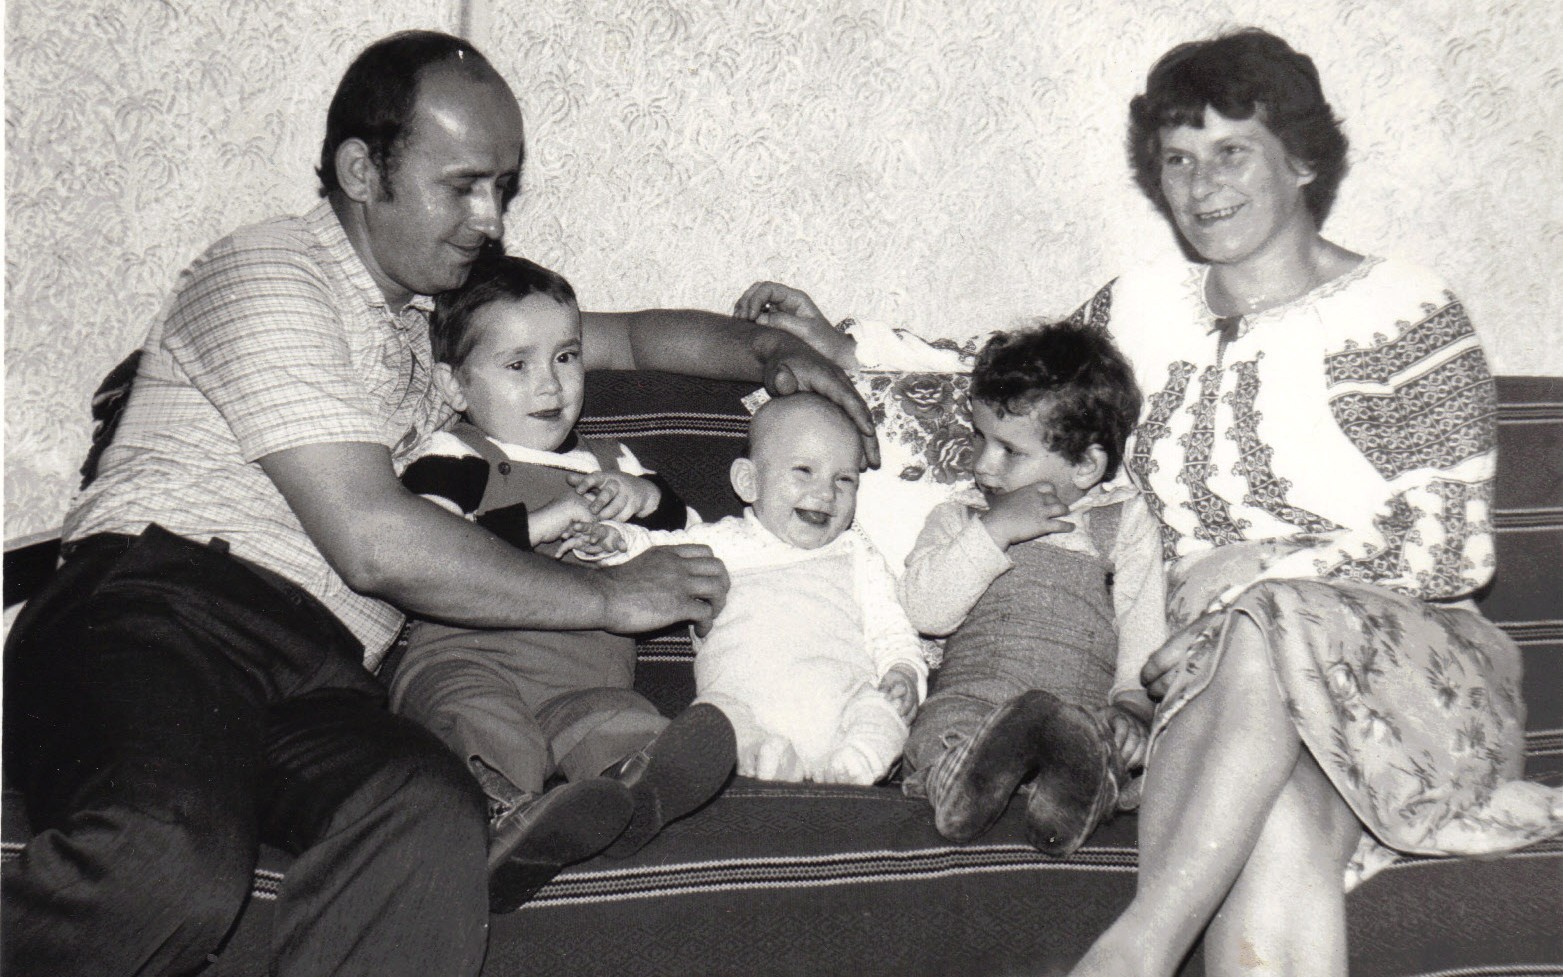
\includegraphics[width=0.7\textwidth]{zdjecia/barbara_i_ryszard_wilk_z_dziecmi.jpg}
\caption[Barbara i Ryszard Wilkowie z dziećmi]{Rodzina Wilków. Od lewej: Ryszard Wilk, jego synowie: Krzysztof i Irek, dalej córka Kasia oraz żona Barbara}
\label{rys:barbara_i_ryszard_wilk_z_dziecmi}
\end{center}
\end{figure}

Barbara Głąbówna wychowywana jak rodzona córka przez Anielę i Karola Biskupskich wyszła dnia 8 V 1976~r. w Kraskowie za Ryszarda Wilka (ur. 2 X 1953~r. w Nysie z ojca Aleksandra i matki Janiny Postrożnej). Ma z nim czwórkę dzieci: Krzysztofa Wilka (ur. 18 VIII 1976~r. w Kluczborku), córkę Katarzynę (ur. 8 III 1980~r. w Kluczborku), syna Ireneusza (ur. 8 I 1982~r. w Namysłowie) oraz najmłodszego Arkadiusza (ur. 18 X 1983~r. w Kluczborku) (ryc.~\ref{rys:barbara_i_ryszard_wilk_z_dziecmi}).

\begin{sidewaysfigure}
\begin{center}
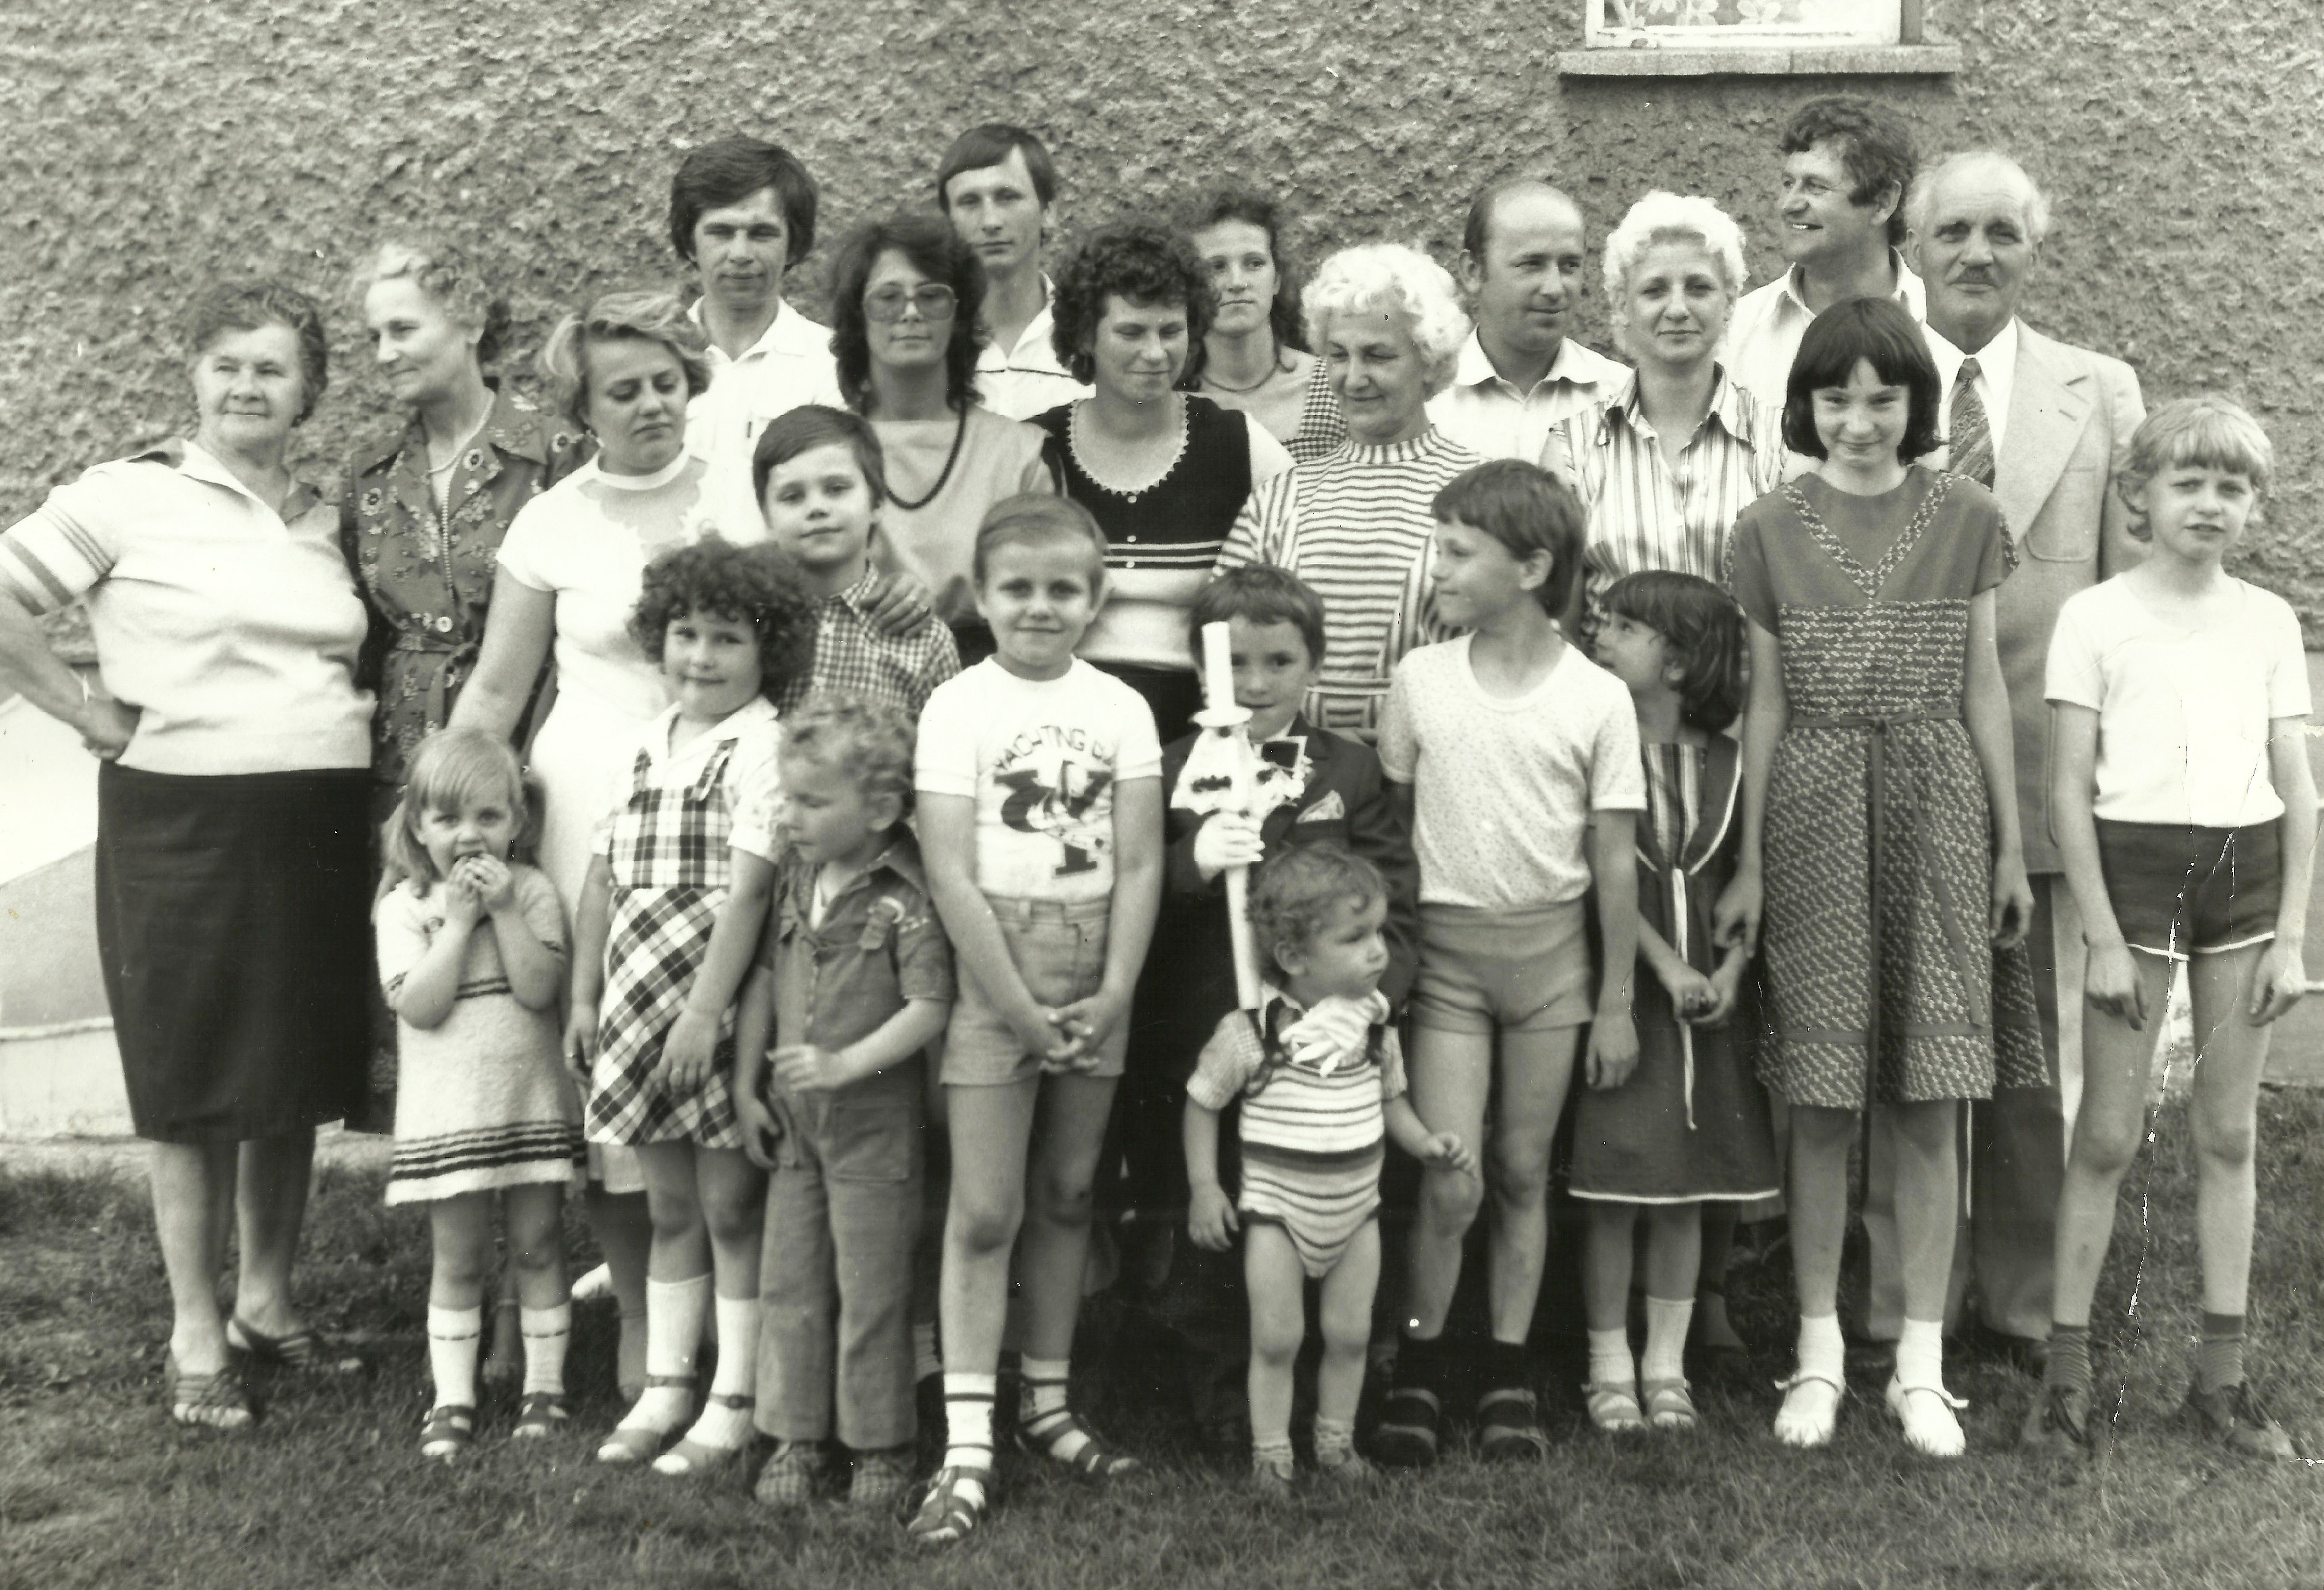
\includegraphics[height=150mm]{zdjecia/komunia_krzysztofa_wilka.jpg}
\caption[Pierwsza komunia św. Krzysztofa Wilka]{Pierwsza komunia św. Krzysztofa Wilka. Na zdj. w I rzędzie dzieci: druga z lewej Kasia Wilk, Irek Wilk, w środku Krzysiu Wilk u I Komunii św. przed nim najmłodszy jego brat Arek, obok Miłosz Głąb, jego siostra Agnieszka, Zuzia Świerczyńska, wyżej od lewej: Aniela Głąb -- Biskupska, w okularach Czesława Świerczyńska, dalej Barbara Wilk (mama), Janina Wilkowa (mama Ryszarda i babka Krzysia), na końcu z prawej Karol Biskupski, w ostatnim rzędzie drugi od lewej Mirosław Głąb, dalej jego żona Elżbieta i Ryszard Wilk (ojciec)}
\label{rys:komunia_krzysztofa_wilka}
\end{center}
\end{sidewaysfigure}


Z tej potężnej gromadki pierwszy Irek założył rodzinę, żeniąc się 28 lipca 2007~r. w Kluczborku z Iwoną Otorowską (ur. 26 X 1983~r. w Kluczborku z ojca Mariana i matki Barbary z Maryniaków), z którą ma dwójkę dzieci: syna Krystiana (ur. 28 XII 2006~r. w Kluczborku) oraz córkę Wiktorię (ur. 7 II 2008~r. w Kluczborku). Po nim Katarzyna Wilk wyszła 20 XII 2012~r. w Kluczborku za Andrzeja Kuźnika (ur. 21 XI 1983~r. w Strzelinie z ojca Ryszarda i matki Heleny Dudek). Najmłodszy Arkadiusz Wilk bierze ślub w Kraskowie 11 VI 2016 r.z Sylwią Szczepańską z Ligoty Dolnej.





\section{Mirosław Głąb}

Mirosław Głąb, jedyny żyjący syn Franciszka pozostał na ojcowiźnie i wybudował w Mirowie dom ,,na ogrodzie''. Ożenił się 19 lutego 1977~r. w Niegowie z Elżbietą Surowiec (ur. 17 V 1958~r. w Mirowie z ojca Antoniego i matki Kazimiery z Męcików) (ryc.~\ref{rys:slub_miroslawa_i_elzbiety_glabow}).

\begin{figure}
\begin{center}
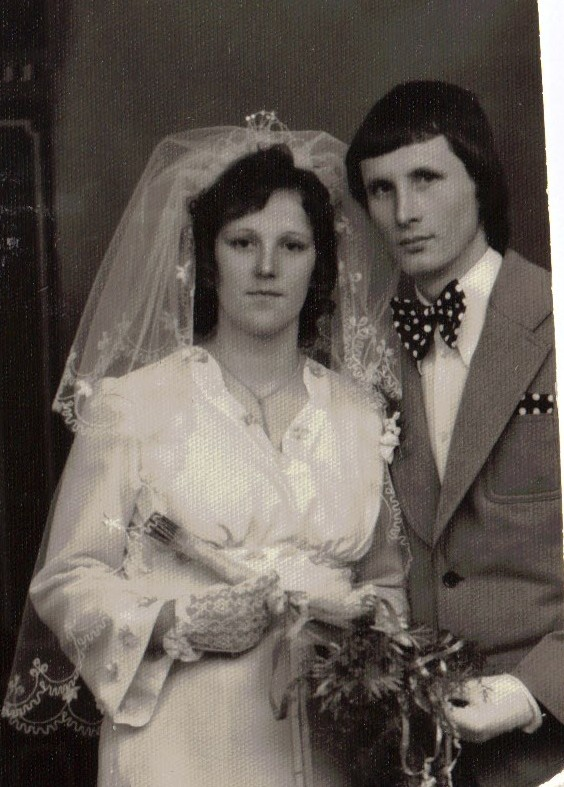
\includegraphics[width=0.45\textwidth]{zdjecia/slub_miroslawa_i_elzbiety_glabow.jpg}
\caption{Ślub Mirosława Głąba z Elżbietą Surowiec}
\label{rys:slub_miroslawa_i_elzbiety_glabow}
\end{center}
\end{figure}

\begin{figure}
\begin{center}
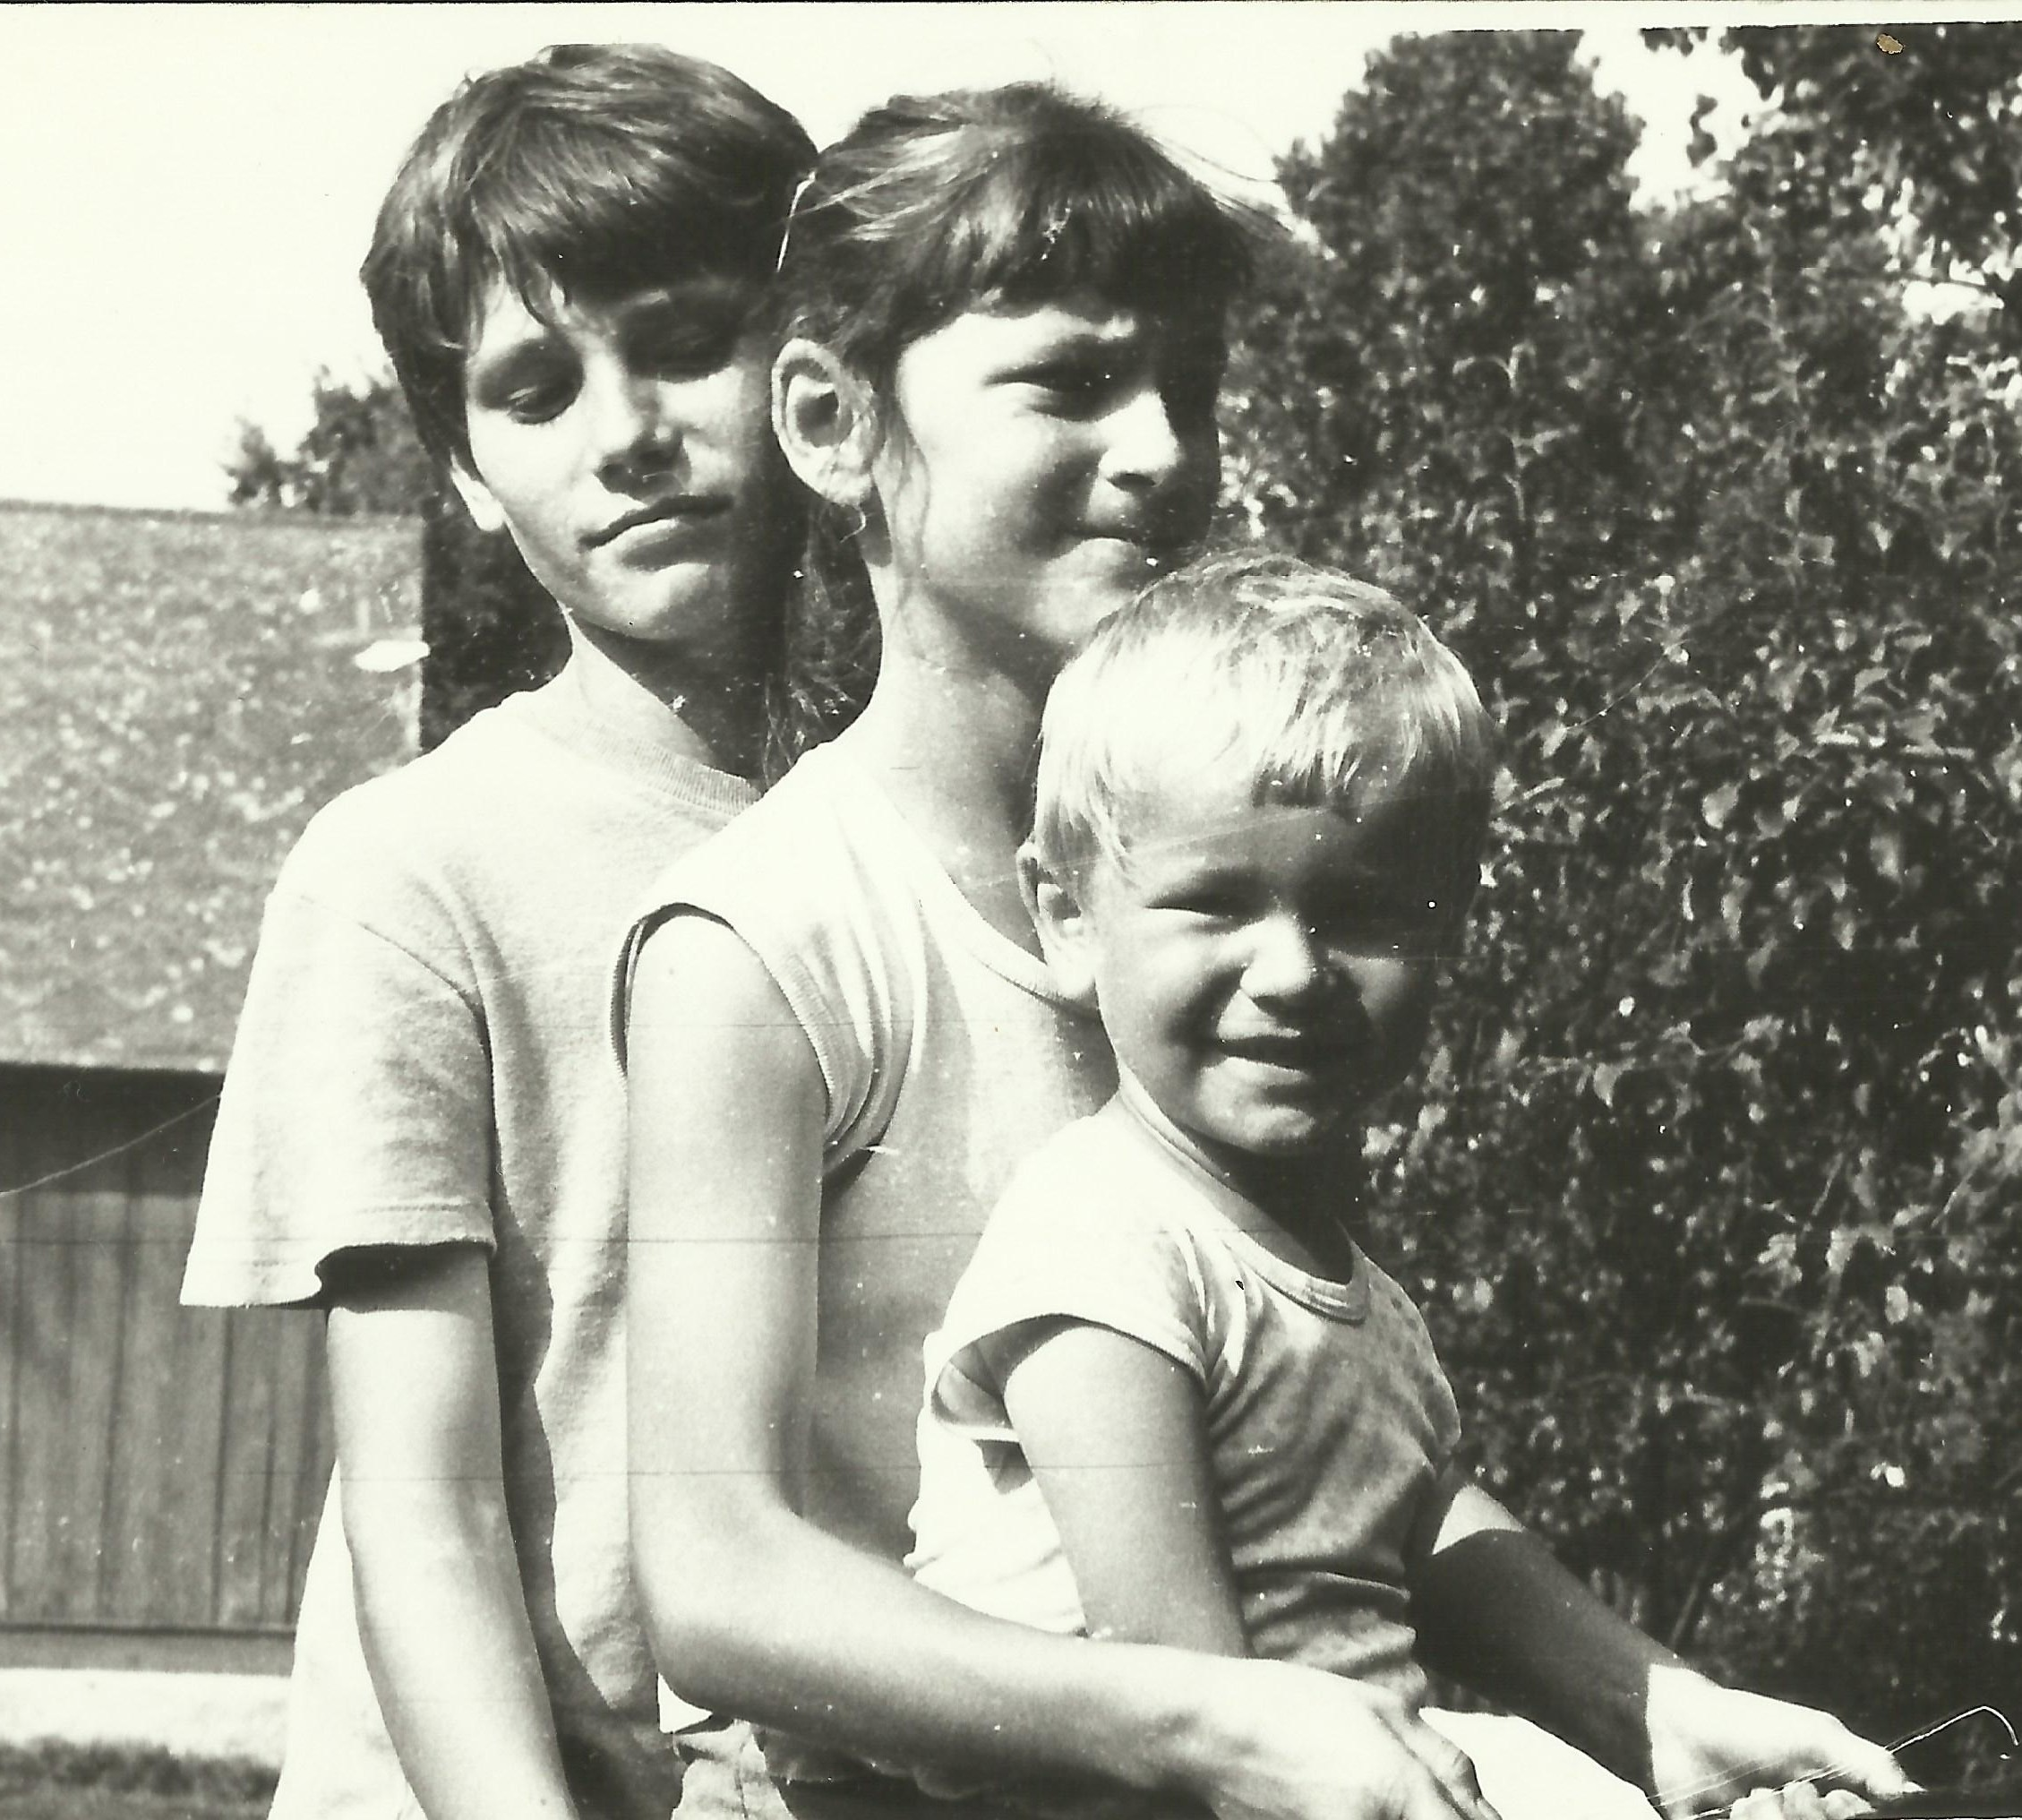
\includegraphics[width=0.6\textwidth]{zdjecia/dzieci_miroslawa_glaba.jpg}
\caption[Miłosz, Agnieszka i Krystian Głąbowie]{Miłosz, Agnieszka i Krystian Głąbowie - dzieci Mirosława i Elżbiety Głąb}
\label{rys:dzieci_miroslawa_glaba}
\end{center}
\end{figure}

Ma z nią troje dzieci: najstarszego Miłosza Głąba (ur. 13 III 1977~r. w Koziegłowach), córkę Agnieszkę (ur. 11 XII 1979~r. w Żarkach) i najmłodszego Krystiana (ur. 3 I 1988~r. w Myszkowie).
Miłosz Głąb ożenił się 14 VI 2014 r. w Krakowie z Martą Ziębą ur. 3 III 1982 r., córką Henryka i Janiny Krupy. Ma z nią córkę Matyldę urodzoną w Krakowie dnia 8 X 2014 r. 
%TODO ***Tu zdj. Miłosza i Marty z Matyldą i z dziadkami.
\begin{sidewaysfigure}
\begin{center}
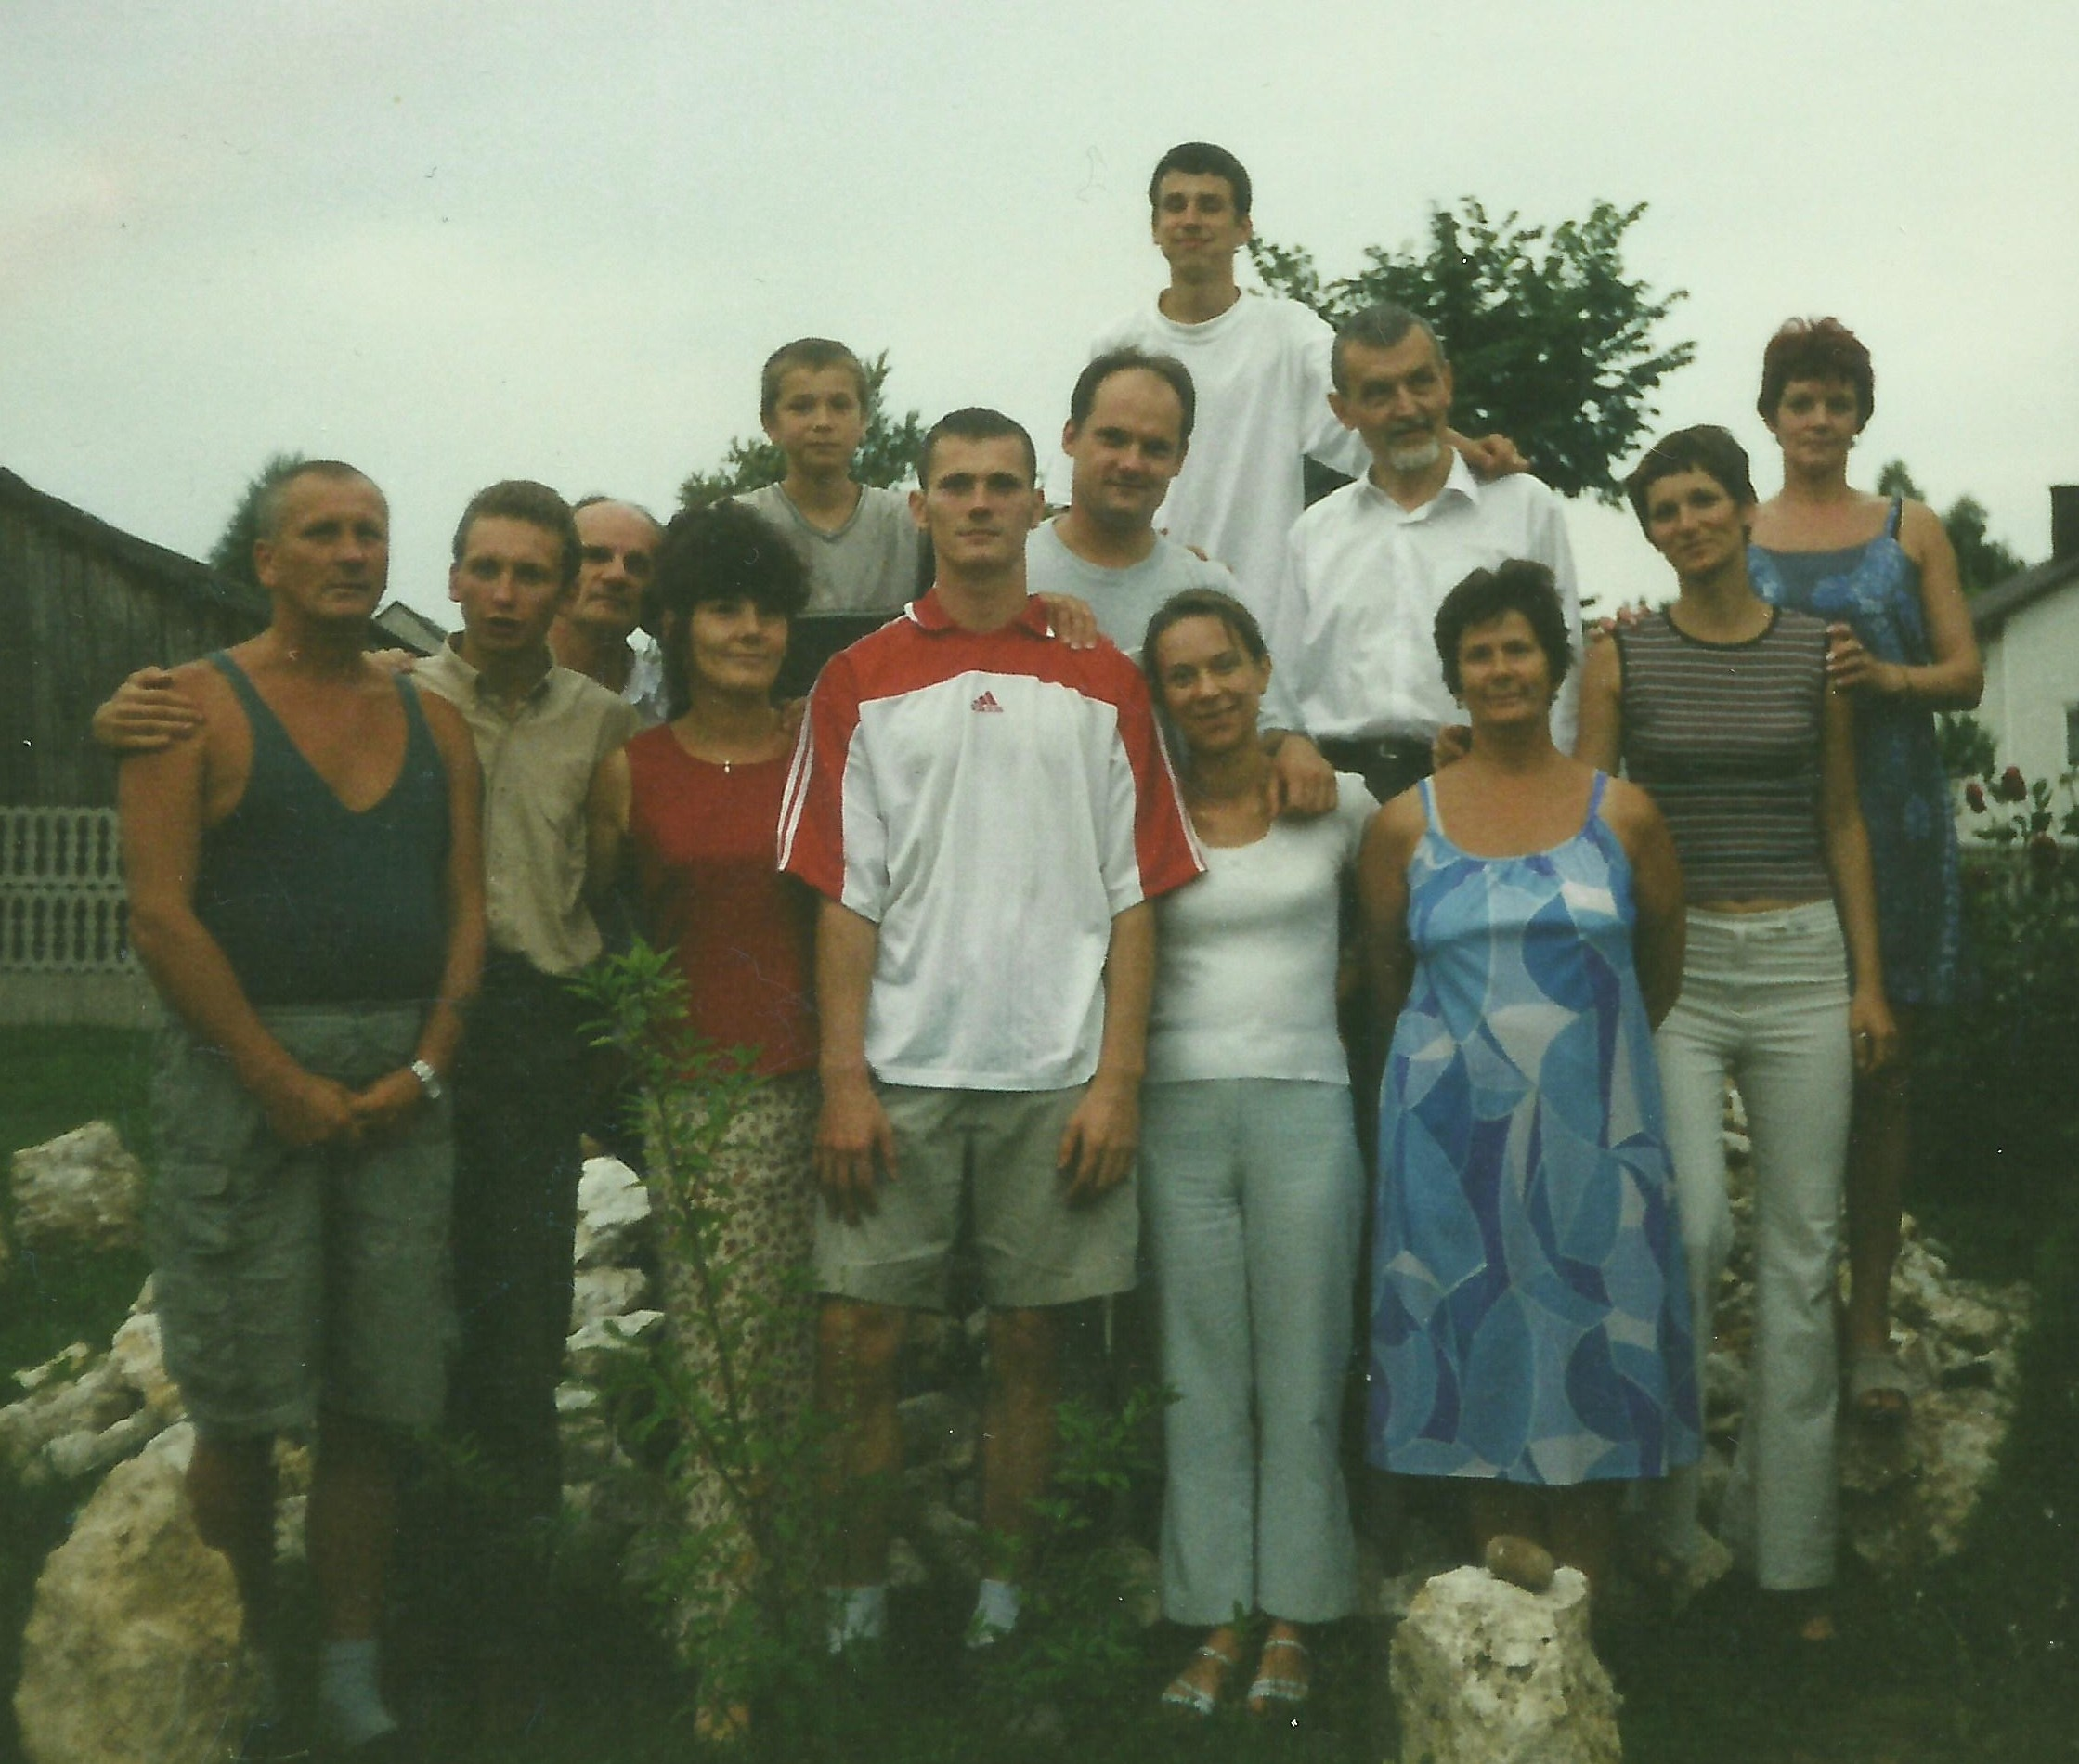
\includegraphics[height=150mm]{zdjecia/rodzina_franciszka_glaba.jpg}
\caption[Zdjęcie zbiorowe rodziny Franciszka Głąba]{Zdjęcie zbiorowe rodziny Franciszka Głąba: najwyżej stoi: Piotr Świerczyński, niżej od lewej: Krystian Głąb, Rafał Jabłoński, Czesław Świerczyński i Halina Czyż z domu Surowiec (siostra Elżbiety Głąbowej), w pierwszym rzędzie od lewej: Mirosław Głąb, Bożydar Świerczyński, Jerzy Jabłoński, Mirosława Jabłońska, Miłosz Głąb, Agnieszka Jabłońska, Czesława Świerczyńska i Agnieszka Głąbówna}
\label{rys:rodzina_franciszka_glaba}
\end{center}
\end{sidewaysfigure}